\documentclass[8pt]{beamer}

\usetheme{metropolis}

\usepackage{amsmath}
\usepackage{bbm}
\usepackage{pgfplots}
\usepackage{hyperref}
\usepackage{listings}
\usepackage{tcolorbox}
\usepackage{xcolor}

\usepgfplotslibrary{groupplots}

\usetikzlibrary{arrows.meta}
\usetikzlibrary{calc}

\hypersetup{
    colorlinks=true,
    linkcolor=blue,
    urlcolor=blue!80
}

\lstdefinestyle{RStyle}{
    language=R,
    basicstyle=\ttfamily\fontsize{5}{6}\selectfont,
    keywordstyle=\color[RGB]{17, 115, 187},
    commentstyle=\color[RGB]{0, 128, 0},
    identifierstyle=\color[RGB]{0, 0, 0},
    stringstyle=\color[RGB]{205, 49, 49},
    numberstyle=\fontsize{5}{6}\selectfont\color[RGB]{128, 128, 128},
    numbers=left,
    numbersep=6pt,
    backgroundcolor=\color[RGB]{255, 255, 255},
    frame=single,
    rulecolor=\color[RGB]{0, 0, 0},
    showstringspaces=false,
    breaklines,
    xleftmargin=3pt,
    xrightmargin=3pt,
    framesep=3pt,
    aboveskip=-1.5pt,
    belowskip=-0.5pt,
    showlines=true
}

\lstdefinestyle{PythonStyle}{
    language=Python,
    basicstyle=\ttfamily\fontsize{5}{6}\selectfont,
    keywordstyle=\color[RGB]{26, 13, 171},
    commentstyle=\color[RGB]{0, 128, 0},
    identifierstyle=\color[RGB]{0, 0, 0},
    stringstyle=\color[RGB]{205, 49, 49},
    numberstyle=\fontsize{5}{6}\selectfont\color[RGB]{128, 128, 128},
    frame=tblr,
    backgroundcolor=\color[RGB]{245, 245, 245},
    rulecolor=\color[RGB]{192, 192, 192},
    showstringspaces=false,
    breaklines,
    xleftmargin=3pt,
    xrightmargin=3pt,
    framesep=3pt,
    aboveskip=-1.5pt,
    belowskip=-0.5pt,
    showlines=true,
}

\lstdefinestyle{ROutput}{
    language=R,
    basicstyle=\ttfamily\fontsize{5}{6}\selectfont,
    backgroundcolor=\color[RGB]{255, 255, 255},
    commentstyle=\color[HTML]{009900},
    stringstyle=\color[HTML]{0000FF},
    keywordstyle=\color[HTML]{000000},
    numberstyle=\tiny\color[HTML]{000000},
    breakatwhitespace=true,
    breaklines=true,
    frame=single,
    rulecolor=\color{black},
    showstringspaces=false,
    breaklines,
    xleftmargin=3pt,
    xrightmargin=3pt,
    framesep=3pt,
    aboveskip=-1.5pt,
    belowskip=-0.5pt,
    showlines=true
}

\lstdefinestyle{PythonOutput}{
    basicstyle=\fontsize{5}{6}\selectfont,
    backgroundcolor=\color[RGB]{255, 255, 255},
    rulecolor=\color[RGB]{192, 192, 192},
    frame=single,
    numbers=none,
    showstringspaces=false,
    breaklines=true,
    breakatwhitespace=true,
    showstringspaces=false,
    breaklines,
    xleftmargin=3pt,
    xrightmargin=3pt,
    framesep=3pt,
    aboveskip=-1.5pt,
    belowskip=-0.5pt,
    showlines=true,
    keywordstyle=\color[RGB]{255, 0, 0},
    morekeywords={AttributeError}
}

\title{PSY9511: Seminar 3}
\subtitle{Variable selection and regularization}
\author{Esten H. Leonardsen}
\date{07.09.23}

\begin{document}
	\begin{frame}
	 	\maketitle
	\end{frame}

    \begin{frame}{Outline}
        \centering
        \vfill
        \begin{enumerate}
            \item Introduction
            \begin{itemize}
                \item Python
                \item Coding tips: Separation of concerns
            \end{itemize}
            \item Regularization
            \begin{itemize}
                \item Variable selection
                \item Shrinkage (+ live coding)
                \item Dimensionality reduction
            \end{itemize}
        \end{enumerate}
        \vfill
    \end{frame}

    \def\codewidth{4.5cm}

    \begin{frame}[fragile]{Python: Imports} % R import
        \centering
        \vfill
        \begin{tikzpicture}
            \node[
                minimum width=\codewidth,
                text width=\codewidth,
                align=left,
                inner sep=0pt,
                outer sep=0pt,
                draw=black
            ] (rcode) at (0, 0) {
                \begin{lstlisting}[style=RStyle, linewidth=\codewidth]




                \end{lstlisting}
            };

            \node[
                draw=black,
                dashed,
                minimum width=\codewidth,
                minimum height=2cm,
                anchor=north,
                text width=\codewidth * 0.98,
                text depth=1.6cm,
                inner sep=0pt,
                outer sep=0pt
            ] (mass) at ($ (rcode.south) - (0, 1.5) $) {\footnotesize{\textbf{MASS}}};

            \node[
                draw=black,
                dashed,
                inner sep=3pt
            ] at (mass) {\scriptsize{lda}};


            \node[] at (-2.35, 0.53) {};
            \node[] at (8.08, -4) {};
        \end{tikzpicture}
        \vfill
    \end{frame}

    \begin{frame}[fragile]{Python: Imports} % R import
        \centering
        \vfill
        \begin{tikzpicture}
            \node[
                minimum width=\codewidth,
                text width=\codewidth,
                align=left,
                inner sep=0pt,
                outer sep=0pt,
                draw=black
            ] (rcode) at (0, 0) {
                \begin{lstlisting}[style=RStyle, linewidth=\codewidth]
library(MASS)



                \end{lstlisting}
            };

            \node[
                draw=black,
                dashed,
                minimum width=\codewidth,
                minimum height=2cm,
                anchor=north,
                text width=\codewidth * 0.98,
                text depth=1.6cm,
                inner sep=0pt,
                outer sep=0pt
            ] (mass) at ($ (rcode.south) - (0, 1.5) $) {\footnotesize{\textbf{MASS}}};

            \node[
                draw=black,
                dashed,
                inner sep=3pt
            ] at (mass) {\scriptsize{lda}};


            \draw[->] (mass.north) -- (rcode.south);
            \node[] at (-2.35, 0.53) {};
            \node[] at (8.08, -4) {};
        \end{tikzpicture}
        \vfill
    \end{frame}

    \begin{frame}[fragile]{Python: Imports} % R import and usage
        \centering
        \vfill
        \begin{tikzpicture}
            \node[
                minimum width=\codewidth,
                text width=\codewidth,
                align=left,
                inner sep=0pt,
                outer sep=0pt,
                draw=black
            ] (rcode) at (0, 0) {
                \begin{lstlisting}[style=RStyle, linewidth=\codewidth]
library(MASS)

lda_fit <- lda(display ~ age + fb,
               data = display)
                \end{lstlisting}
            };

            \node[
                draw=black,
                dashed,
                minimum width=\codewidth,
                minimum height=2cm,
                anchor=north,
                text width=\codewidth * 0.98,
                text depth=1.6cm,
                inner sep=0pt,
                outer sep=0pt
            ] (mass) at ($ (rcode.south) - (0, 1.5) $) {\footnotesize{\textbf{MASS}}};

            \node[
                draw=black,
                dashed,
                inner sep=3pt
            ] at (mass) {\scriptsize{lda}};


            \draw[->] (mass.north) -- (rcode.south);
            \node[] at (-2.35, 0.53) {};
            \node[] at (8.08, -4) {};
        \end{tikzpicture}
        \vfill
    \end{frame}

    \begin{frame}[fragile]{Python: Imports} % Import everything from package
        \centering
        \vfill
        \begin{tikzpicture}
            \node[
                minimum width=\codewidth,
                text width=\codewidth,
                align=left,
                inner sep=0pt,
                outer sep=0pt,
                draw=black
            ] (rcode) at (0, 0) {
                \begin{lstlisting}[style=RStyle, linewidth=\codewidth]
library(MASS)

lda_fit <- lda(display ~ age + fb,
               data = display)
                \end{lstlisting}
            };
            \node[
                minimum width=\codewidth,
                text width=\codewidth,
                align=left,
                inner sep=0pt,
                outer sep=0pt,
                anchor=north west,
                draw=black,
                label={[blue,
                        anchor=north east,
                        font=\ttfamily\fontsize{5}{6}\selectfont,
                        inner sep=0pt,
                        outer sep=0pt,
                        xshift=-3pt,
                        yshift=-3pt,
                        text depth=0
                       ]north west:In{[}1{]}:},
            ] (pythoncode) at ($ (rcode.north east) + (1.4, 0) $) {
                \begin{lstlisting}[style=PythonStyle, linewidth=\codewidth]
from sklearn import *

lda = discriminant_analysis.LinearDiscriminantAnalysis()
lda.fit(display[['age', 'fb']],
        display['display'])
                \end{lstlisting}
            };

            \node[
                draw=black,
                dashed,
                minimum width=\codewidth,
                minimum height=2cm,
                anchor=north,
                text width=\codewidth * 0.98,
                text depth=1.6cm,
                inner sep=0pt,
                outer sep=0pt
            ] (mass) at ($ (rcode.south) - (0, 1.5) $) {\footnotesize{\textbf{MASS}}};

            \node[
                draw=black,
                dashed,
                inner sep=3pt
            ] at (mass) {\scriptsize{lda}};

            \node[
                draw=black,
                dashed,
                minimum width=\codewidth,
                minimum height=2cm,
                anchor=west,
                text width=\codewidth * 0.98,
                text depth=1.6cm,
                inner sep=0pt,
                outer sep=0pt,
            ] (sklearn) at ($ (mass.east) + (1.4, 0) $) {\footnotesize{\textbf{sklearn}}};

            \node[
                draw=black,
                dashed,
                minimum width=\codewidth * 0.8,
                minimum height=1.3cm,
                text width=\codewidth * 0.78,
                text depth=0.97cm,
                inner sep=0pt,
                outer sep=0pt,
                anchor=south
            ] (da) at ($ (sklearn.south) + (0, 0.15) $) {\scriptsize{\textbf{discriminant\_analysis}}};

            \node[
                draw=black,
                dashed,
                inner sep=2pt,
                anchor=south
            ] (lda) at ($ (da.south) + (0, 0.15) $) {\tiny{LinearDiscriminantAnalysis}};

            \draw[->] (mass.north) -- (rcode.south);
            \draw[->] (sklearn.north) -- (pythoncode.south);
            \node[] at (-2.35, 0.53) {};
            \node[] at (8.08, -4) {};
        \end{tikzpicture}
        \vfill
    \end{frame}

    \begin{frame}[fragile]{Python: Imports} % Import entire package
        \centering
        \vfill
        \begin{tikzpicture}
            \node[
                minimum width=\codewidth,
                text width=\codewidth,
                align=left,
                inner sep=0pt,
                outer sep=0pt,
                draw=black
            ] (rcode) at (0, 0) {
                \begin{lstlisting}[style=RStyle, linewidth=\codewidth]
library(MASS)

lda_fit <- lda(display ~ age + fb,
               data = display)
                \end{lstlisting}
            };
            \node[
                minimum width=\codewidth,
                text width=\codewidth,
                align=left,
                inner sep=0pt,
                outer sep=0pt,
                anchor=north west,
                draw=black,
                label={[blue,
                        anchor=north east,
                        font=\ttfamily\fontsize{5}{6}\selectfont,
                        inner sep=0pt,
                        outer sep=0pt,
                        xshift=-3pt,
                        yshift=-3pt
                       ]north west:In{[}1{]}:},
            ] (pythoncode) at ($ (rcode.north east) + (1.4, 0) $) {
                \begin{lstlisting}[style=PythonStyle, linewidth=\codewidth]
import sklearn

lda = sklearn.discriminant_analysis.LinearDiscriminantAnalysis()
lda.fit(display[['age', 'fb']],
        display['display'])
                \end{lstlisting}
            };

            \node[
                draw=black,
                dashed,
                minimum width=\codewidth,
                minimum height=2cm,
                anchor=north,
                text width=\codewidth * 0.98,
                text depth=1.6cm,
                inner sep=0pt,
                outer sep=0pt
            ] (mass) at ($ (rcode.south) - (0, 1.5) $) {\footnotesize{\textbf{MASS}}};

            \node[
                draw=black,
                dashed,
                inner sep=3pt
            ] at (mass) {\scriptsize{lda}};

            \node[
                draw=black,
                dashed,
                minimum width=\codewidth,
                minimum height=2cm,
                anchor=west,
                text width=\codewidth * 0.98,
                text depth=1.6cm,
                inner sep=0pt,
                outer sep=0pt
            ] (sklearn) at ($ (mass.east) + (1.4, 0) $) {\footnotesize{\textbf{sklearn}}};

            \node[
                draw=black,
                dashed,
                minimum width=\codewidth * 0.8,
                minimum height=1.3cm,
                text width=\codewidth * 0.78,
                text depth=0.97cm,
                inner sep=0pt,
                outer sep=0pt,
                anchor=south
            ] (da) at ($ (sklearn.south) + (0, 0.15) $) {\scriptsize{\textbf{discriminant\_analysis}}};

            \node[
                draw=black,
                dashed,
                inner sep=2pt,
                anchor=south
            ] (lda) at ($ (da.south) + (0, 0.15) $) {\tiny{LinearDiscriminantAnalysis}};

            \draw[->] (mass.north) -- (rcode.south);
            \draw[->] (sklearn.north) -- (pythoncode.south);
            \draw[densely dotted] (lda.north) -- (sklearn.north);
            \node[] at (-2.35, 0.53) {};
            \node[] at (8.08, -4) {};
        \end{tikzpicture}
        \vfill
    \end{frame}

    \begin{frame}[fragile]{Python: Imports} % Proper import
        \centering
        \vfill
        \begin{tikzpicture}
            \node[
                minimum width=\codewidth,
                text width=\codewidth,
                align=left,
                inner sep=0pt,
                outer sep=0pt,
                draw=black
            ] (rcode) at (0, 0) {
                \begin{lstlisting}[style=RStyle, linewidth=\codewidth]
library(MASS)

lda_fit <- lda(display ~ age + fb,
               data = display)
                \end{lstlisting}
            };
            \node[
                minimum width=\codewidth,
                text width=\codewidth,
                align=left,
                inner sep=0pt,
                outer sep=0pt,
                anchor=north west,
                label={[blue,
                        anchor=north east,
                        font=\ttfamily\fontsize{5}{6}\selectfont,
                        inner sep=0pt,
                        outer sep=0pt,
                        xshift=-3pt,
                        yshift=-3pt
                       ]north west:In{[}1{]}:},
            ] (pythoncode) at ($ (rcode.north east) + (1.4, 0) $) {
                \begin{lstlisting}[style=PythonStyle, linewidth=\codewidth]
from sklearn.discriminant_analysis \
    import LinearDiscriminantAnalysis

lda = LinearDiscriminantAnalysis()
lda.fit(display[['age', 'fb']],
        display['display'])
                \end{lstlisting}
            };

            \node[
                draw=black,
                dashed,
                minimum width=\codewidth,
                minimum height=2cm,
                anchor=north,
                text width=\codewidth * 0.98,
                text depth=1.6cm,
                inner sep=0pt,
                outer sep=0pt
            ] (mass) at ($ (rcode.south) - (0, 1.5) $) {\footnotesize{\textbf{MASS}}};

            \node[
                draw=black,
                dashed,
                inner sep=3pt
            ] at (mass) {\scriptsize{lda}};

            \node[
                draw=black,
                dashed,
                minimum width=\codewidth,
                minimum height=2cm,
                anchor=west,
                text width=\codewidth * 0.98,
                text depth=1.6cm,
                inner sep=0pt,
                outer sep=0pt
            ] (sklearn) at ($ (mass.east) + (1.4, 0) $) {\footnotesize{\textbf{sklearn}}};

            \node[
                draw=black,
                dashed,
                minimum width=\codewidth * 0.8,
                minimum height=1.3cm,
                text width=\codewidth * 0.78,
                text depth=0.97cm,
                inner sep=0pt,
                outer sep=0pt,
                anchor=south
            ] (da) at ($ (sklearn.south) + (0, 0.15) $) {\scriptsize{\textbf{discriminant\_analysis}}};

            \node[
                draw=black,
                dashed,
                inner sep=2pt,
                anchor=south
            ] (lda) at ($ (da.south) + (0, 0.15) $) {\tiny{LinearDiscriminantAnalysis}};

            \draw[->] (mass.north) -- (rcode.south);
            \draw[->] (lda.north) -- (pythoncode.south);
            \node[] at (-2.35, 0.53) {};
            \node[] at (8.08, -4) {};
        \end{tikzpicture}
        \vfill
    \end{frame}

    \def\codewidth{4.8cm}

    \begin{frame}[fragile]{Python: pandas}
        \centering
        \vfill
        \begin{tikzpicture}
            \node[
                minimum width=\codewidth,
                text width=\codewidth,
                align=left,
                inner sep=0pt,
                outer sep=0pt,
                draw=black,
            ] (rcode) at (0, 0) {
                \begin{lstlisting}[style=RStyle]
path <- '/Users/esten/Downloads/Auto.csv'
df <- read.csv(path)
head(df, 10)
                \end{lstlisting}
            };
            \node[
                minimum width=\codewidth,
                text width=\codewidth,
                align=left,
                inner sep=0pt,
                outer sep=0pt,
                anchor=north west,
                draw=black,
                label={[blue,
                        anchor=north east,
                        font=\ttfamily\fontsize{5}{6}\selectfont,
                        inner sep=0pt,
                        outer sep=0pt,
                        xshift=-3pt,
                        yshift=-3pt
                       ]north west:In{[}1{]}:}
            ] (pythoncode) at ($ (rcode.north east) + (1.2, 0) $) {
                \begin{lstlisting}[style=PythonStyle]
import pandas as pd

path = '/Users/esten/Downloads/Auto.csv'
df = pd.read_csv(path)
df.head(10)
                \end{lstlisting}
            };

            \node[
                minimum width=\codewidth,
                text width=\codewidth,
                align=left,
                inner sep=0pt,
                outer sep=0pt,
                anchor=north,
            ] (routput) at ($ (rcode.south) - (0, 1) $) {
                \begin{lstlisting}[style=ROutput]
     mpg cylinders displacement horsepower
1    18         8        307.0        130
2    15         8        350.0        165
3    18         8        318.0        150
4    16         8        304.0        150
5    17         8        302.0        140
6    15         8        429.0        198
7    14         8        454.0        220
8    14         8        440.0        215
9    14         8        455.0        225
10   15         8        390.0        190
                \end{lstlisting}
            };

            \node[
                minimum width=\codewidth,
                text width=\codewidth,
                align=left,
                inner sep=0pt,
                outer sep=0pt,
                anchor=north west,
                label={[red,
                        anchor=north east,
                        font=\ttfamily\fontsize{5}{6}\selectfont,
                        inner sep=0pt,
                        outer sep=0pt,
                        xshift=-3pt,
                        yshift=-3pt
                        ]north west:Out{[}1{]}:}
            ] (pythonoutput) at ($ (routput.north east) + (1.2, 0) $) {
                \begin{lstlisting}[style=PythonOutput]
     mpg cylinders displacement horsepower
0    18         8        307.0        130
1    15         8        350.0        165
2    18         8        318.0        150
3    16         8        304.0        150
4    17         8        302.0        140
5    15         8        429.0        198
6    14         8        454.0        220
7    14         8        440.0        215
8    14         8        455.0        225
9    15         8        390.0        190
                \end{lstlisting}
            };
        \end{tikzpicture}
        \vfill
    \end{frame}

    \def\codewidth{9cm}

    \begin{frame}[fragile]{Python: numpy}
        \centering
        \vfill
        \begin{tikzpicture}
            \node[
                minimum width=\codewidth,
                text width=\codewidth,
                align=left,
                inner sep=0pt,
                outer sep=0pt,
                draw=black,
                label={[blue,
                        anchor=north east,
                        font=\ttfamily\fontsize{5}{6}\selectfont,
                        inner sep=0pt,
                        outer sep=0pt,
                        xshift=-3pt,
                        yshift=-3.5pt,
                        text depth=0
                       ]north west:In{[}1{]}:}
            ] (code0) at (0, 0) {
                \begin{lstlisting}[style=PythonStyle]
import numpy as np
                \end{lstlisting}
            };

            \node[
                minimum width=\codewidth,
                text width=\codewidth,
                align=left,
                inner sep=0pt,
                anchor=north,
                label={[blue,
                        anchor=north east,
                        font=\ttfamily\fontsize{5}{6}\selectfont,
                        inner sep=0pt,
                        outer sep=0pt,
                        xshift=-3pt,
                        yshift=-3.5pt,
                        text depth=0
                       ]north west:In{[}2{]}:}
            ] (code1) at ($ (code0.south) - (0, 0.1) $) {
                \begin{lstlisting}[style=PythonStyle]
np.random.seed(42)
                \end{lstlisting}
            };

            \node[
                minimum width=\codewidth,
                text width=\codewidth,
                align=left,
                inner sep=0pt,
                anchor=north,
                label={[blue,
                        anchor=north east,
                        font=\ttfamily\fontsize{5}{6}\selectfont,
                        inner sep=0pt,
                        outer sep=0pt,
                        xshift=-3pt,
                        yshift=-3.5pt,
                        text depth=0
                       ]north west:In{[}3{]}:}
            ] (code2) at ($ (code1.south) - (0, 0.1) $) {
                \begin{lstlisting}[style=PythonStyle]
np.arange(0, 10, 1)
                \end{lstlisting}
            };

            \node[
                minimum width=\codewidth,
                text width=\codewidth,
                align=left,
                inner sep=0pt,
                anchor=north,
                label={[red,
                        anchor=north east,
                        font=\ttfamily\fontsize{5}{6}\selectfont,
                        inner sep=0pt,
                        outer sep=0pt,
                        xshift=-3pt,
                        yshift=-3.5pt,
                        text depth=0
                        ]north west:Out{[}1{]}:}
            ] (code3) at ($ (code2.south) - (0, 0.1) $) {
                \begin{lstlisting}[style=PythonOutput]
array([0, 1, 2, 3, 4, 5, 6, 7, 8, 9])
                \end{lstlisting}
            };

            \node[
                minimum width=\codewidth,
                text width=\codewidth,
                align=left,
                inner sep=0pt,
                anchor=north,
                label={[blue,
                        anchor=north east,
                        font=\ttfamily\fontsize{5}{6}\selectfont,
                        inner sep=0pt,
                        outer sep=0pt,
                        xshift=-3pt,
                        yshift=-3.5pt,
                        text depth=0
                       ]north west:In{[}4{]}:}
            ] (code4) at ($ (code3.south) - (0, 0.1) $) {
                \begin{lstlisting}[style=PythonStyle]
np.isnan([0, 1, np.nan, 3])
                \end{lstlisting}
            };

            \node[
                minimum width=\codewidth,
                text width=\codewidth,
                align=left,
                inner sep=0pt,
                anchor=north,
                label={[red,
                        anchor=north east,
                        font=\ttfamily\fontsize{5}{6}\selectfont,
                        inner sep=0pt,
                        outer sep=0pt,
                        xshift=-3pt,
                        yshift=-3.5pt,
                        text depth=0
                        ]north west:Out{[}2{]}:}
            ] (code5) at ($ (code4.south) - (0, 0.1) $) {
                \begin{lstlisting}[style=PythonOutput]
array([False, False,  True, False])
                \end{lstlisting}
            };

            \node[
                minimum width=\codewidth,
                text width=\codewidth,
                align=left,
                inner sep=0pt,
                anchor=north,
                label={[blue,
                        anchor=north east,
                        font=\ttfamily\fontsize{5}{6}\selectfont,
                        inner sep=0pt,
                        outer sep=0pt,
                        xshift=-3pt,
                        yshift=-3.5pt,
                        text depth=0
                       ]north west:In{[}5{]}:}
            ] (code6) at ($ (code5.south) - (0, 0.1) $) {
                \begin{lstlisting}[style=PythonStyle]
np.amin([1, 0, 3, 2])
                \end{lstlisting}
            };

            \node[
                minimum width=\codewidth,
                text width=\codewidth,
                align=left,
                inner sep=0pt,
                anchor=north,
                label={[red,
                        anchor=north east,
                        font=\ttfamily\fontsize{5}{6}\selectfont,
                        inner sep=0pt,
                        outer sep=0pt,
                        xshift=-3pt,
                        yshift=-3.5pt,
                        text depth=0
                        ]north west:Out{[}3{]}:}
            ] (code7) at ($ (code6.south) - (0, 0.1) $) {
                \begin{lstlisting}[style=PythonOutput]
0
                \end{lstlisting}
            };

            \node[
                minimum width=\codewidth,
                text width=\codewidth,
                align=left,
                inner sep=0pt,
                anchor=north,
                label={[blue,
                        anchor=north east,
                        font=\ttfamily\fontsize{5}{6}\selectfont,
                        inner sep=0pt,
                        outer sep=0pt,
                        xshift=-3pt,
                        yshift=-3.5pt,
                        text depth=0
                        ]north west:Out{[}6{]}:}
            ] (code8) at ($ (code7.south) - (0, 0.1) $) {
                \begin{lstlisting}[style=PythonStyle]
np.argmin([1, 0, 3, 2])
                \end{lstlisting}
            };

            \node[
                minimum width=\codewidth,
                text width=\codewidth,
                align=left,
                inner sep=0pt,
                anchor=north,
                label={[red,
                        anchor=north east,
                        font=\ttfamily\fontsize{5}{6}\selectfont,
                        inner sep=0pt,
                        outer sep=0pt,
                        xshift=-3pt,
                        yshift=-3.5pt,
                        text depth=0
                        ]north west:Out{[}4{]}:}
            ] (code9) at ($ (code8.south) - (0, 0.1) $) {
                \begin{lstlisting}[style=PythonOutput]
1
                \end{lstlisting}
            };

            \node[
                minimum width=\codewidth,
                text width=\codewidth,
                align=left,
                inner sep=0pt,
                anchor=north,
                label={[blue,
                        anchor=north east,
                        font=\ttfamily\fontsize{5}{6}\selectfont,
                        inner sep=0pt,
                        outer sep=0pt,
                        xshift=-3pt,
                        yshift=-3.5pt,
                        text depth=0
                        ]north west:In{[}7{]}:}
            ] (code10) at ($ (code9.south) - (0, 0.1) $) {
                \begin{lstlisting}[style=PythonStyle]
np.nanmin([1, 0, 3, np.nan])
                \end{lstlisting}
            };

            \node[
                minimum width=\codewidth,
                text width=\codewidth,
                align=left,
                inner sep=0pt,
                anchor=north,
                label={[red,
                        anchor=north east,
                        font=\ttfamily\fontsize{5}{6}\selectfont,
                        inner sep=0pt,
                        outer sep=0pt,
                        xshift=-3pt,
                        yshift=-3.5pt,
                        text depth=0
                        ]north west:Out{[}5{]}:}
            ] (code11) at ($ (code10.south) - (0, 0.1) $) {
                \begin{lstlisting}[style=PythonOutput]
0
                \end{lstlisting}
            };
        \end{tikzpicture}
        \vfill
    \end{frame}

    \def\codewidth{5.2cm}

    \begin{frame}[fragile]{Python: statsmodels}
        \begin{tikzpicture}
            \node[
                minimum width=\codewidth,
                text width=\codewidth,
                align=left,
                inner sep=0pt,
                outer sep=0pt,
                draw=black
            ] (rcode) at (0, 0) {
                \begin{lstlisting}[style=RStyle, linewidth=\codewidth]
path <- '/Users/esten/Downloads/Auto.csv'
data <- read.csv(path)

model <- lm(mpg ~ cylinders + displacement +
                  horsepower + weight +
                  acceleration + year,
            data=data)
summary(model)
                \end{lstlisting}
            };

            \node[
                minimum width=\codewidth,
                text width=\codewidth,
                align=left,
                inner sep=0pt,
                outer sep=0pt,
                anchor=north
            ] (routput) at ($ (rcode.south)  - (0, 1.5) $) {
                \begin{lstlisting}[style=ROutput, linewidth=\codewidth]
Coefficients:
                Estimate Std. Error Pr(>|t|)
(Intercept)  -1.454e+01  4.764e+00  0.00244 **
cylinders    -3.299e-01  3.321e-01  0.32122
displacement  7.678e-03  7.358e-03  0.29733
horsepower   -3.914e-04  1.384e-02  0.97745
weight       -6.795e-03  6.700e-04  < 2e-16 ***
acceleration  8.527e-02  1.020e-01  0.40383
year          7.534e-01  5.262e-02  < 2e-16 ***
---
Signif. codes:  0 ‘***’ 0.001 ‘**’ 0.01 ‘*’ 0.05
                \end{lstlisting}
            };

            \node[
                minimum width=\codewidth,
                text width=\codewidth,
                align=left,
                inner sep=0pt,
                outer sep=0pt,
                anchor=north west,
                draw=black,
                label={[blue,
                        anchor=north east,
                        font=\ttfamily\fontsize{5}{6}\selectfont,
                        inner sep=0pt,
                        outer sep=0pt,
                        xshift=-3pt,
                        yshift=-3pt
                       ]north west:In{[}1{]}:},
            ] (pythoncode) at ($ (rcode.north east) + (1, 0) $) {
                \begin{lstlisting}[style=PythonStyle, linewidth=\codewidth]
import statsmodels.formula.api as smf

path = '/Users/esten/Downloads/Auto.csv'
df = pd.read_csv(path)

model = smf.ols(
    formula='mpg ~ cylinders + displacement +'
                   'horsepower + weight + '
                   'acceleration + year',
    data=df
)
fit = model.fit()
print(fit.summary())
                \end{lstlisting}
            };

            \node[
                minimum width=\codewidth,
                text width=\codewidth,
                align=left,
                inner sep=0pt,
                anchor=north west,
                label={[red,
                        anchor=north east,
                        font=\ttfamily\fontsize{5}{6}\selectfont,
                        inner sep=0pt,
                        outer sep=0pt,
                        xshift=-3pt,
                        yshift=-3.5pt,
                        text depth=0
                        ]north west:Out{[}1{]}:}
            ] (pythonout) at ($ (routput.north east) + (1, 0) $) {
                \begin{lstlisting}[style=PythonOutput]
coef  std err  P>|t|  [0.025 0.975]
-----------------------------------------------
Intercept    -14.5353 4.764 0.002 -23.90 -5.16
cylinders    -0.3299  0.332 0.321  -0.98  0.32
displacement  0.0077  0.007 0.297  -0.00  0.02
horsepower   -0.0004  0.014 0.977  -0.02  0.02
weight       -0.0068  0.001 0.000  -0.00 -0.00
acceleration  0.0853  0.102 0.404  -0.11  0.28
year          0.7534  0.053 0.000   0.65  0.85
===============================================
                \end{lstlisting}
            };

        \end{tikzpicture}
    \end{frame}

    \def\codewidth{9cm}

    \begin{frame}[fragile]{Python: scikit-learn} % Similar to statsmodels
        \begin{tikzpicture}
            \node[
                minimum width=\codewidth,
                text width=\codewidth,
                align=left,
                inner sep=0pt,
                anchor=north,
                label={[blue,
                        anchor=north east,
                        font=\ttfamily\fontsize{5}{6}\selectfont,
                        inner sep=0pt,
                        outer sep=0pt,
                        xshift=-3pt,
                        yshift=-3.5pt,
                        text depth=0
                        ]north west:In{[}1{]}:}
            ] (code) at (0, 0) {
                \begin{lstlisting}[style=PythonStyle]
from sklearn.linear_model import LinearRegression

path = '/Users/esten/Downloads/Auto.csv'
df = pd.read_csv(path)

predictors = ['cylinders', 'displacement', 'horsepower',
              'weight', 'acceleration', 'year']
target = 'mpg'

model = LinearRegression()
model.fit(df[predictors], df[target])
model.summary()
                \end{lstlisting}
            };
            \node[] at (4.4, -6.8) {};
            \node[] at (-5.4, -0.1) {};
        \end{tikzpicture}
    \end{frame}

    \begin{frame}[fragile]{Python: scikit-learn} % Error
        \begin{tikzpicture}
            \node[
                minimum width=\codewidth,
                text width=\codewidth,
                align=left,
                inner sep=0pt,
                anchor=north,
                label={[blue,
                        anchor=north east,
                        font=\ttfamily\fontsize{5}{6}\selectfont,
                        inner sep=0pt,
                        outer sep=0pt,
                        xshift=-3pt,
                        yshift=-3.5pt,
                        text depth=0
                        ]north west:In{[}1{]}:}
            ] (code) at (0, 0) {
                \begin{lstlisting}[style=PythonStyle]
from sklearn.linear_model import LinearRegression

path = '/Users/esten/Downloads/Auto.csv'
df = pd.read_csv(path)

predictors = ['cylinders', 'displacement', 'horsepower',
              'weight', 'acceleration', 'year']
target = 'mpg'

model = LinearRegression()
model.fit(df[predictors], df[target])
model.summary()
                \end{lstlisting}
            };

            \node[
                minimum width=\codewidth,
                text width=\codewidth,
                align=left,
                inner sep=0pt,
                anchor=north,
                label={[red,
                        anchor=north east,
                        font=\ttfamily\fontsize{5}{6}\selectfont,
                        inner sep=0pt,
                        outer sep=0pt,
                        xshift=-3pt,
                        yshift=-3.5pt,
                        text depth=0
                        ]north west:Out{[}1{]}:}
            ] (output) at ($ (code.south) - (0, 0.2) $) {
                \begin{lstlisting}[style=PythonOutput]
---------------------------------------------------------------------------
AttributeError                            Traceback (most recent call last)
Cell In[52], line 13
        11 model = LinearRegression()
        12 model.fit(df[predictors], df[target])
---> 13 model.summary()

AttributeError: 'LinearRegression' object has no attribute 'summary'
                \end{lstlisting}
            };
            \node[] at (4.4, -6.8) {};
            \node[] at (-5.4, -0.1) {};
        \end{tikzpicture}
    \end{frame}

    \begin{frame}[fragile]{Python: scikit-learn} % Proper usage
        \begin{tikzpicture}
            \node[
                minimum width=\codewidth,
                text width=\codewidth,
                align=left,
                inner sep=0pt,
                anchor=north,
                label={[blue,
                        anchor=north east,
                        font=\ttfamily\fontsize{5}{6}\selectfont,
                        inner sep=0pt,
                        outer sep=0pt,
                        xshift=-3pt,
                        yshift=-3.5pt,
                        text depth=0
                        ]north west:In{[}1{]}:}
            ] (code) at (0, 0) {
                \begin{lstlisting}[style=PythonStyle]
from sklearn.linear_model import LinearRegression

path = '/Users/esten/Downloads/Auto.csv'
df = pd.read_csv(path)

predictors = ['cylinders', 'displacement', 'horsepower',
              'weight', 'acceleration', 'year']
target = 'mpg'

model = LinearRegression()
model.fit(df[predictors], df[target])

# Print model coefficients
print(f'Intercept: {model.intercept_}')
print(f'Coefficients: {model.coef_}')

# Print model residuals
predictions = model.predict(df[predictors])
residuals = df[target] - predictions
print(f'Residuals: {residuals.values[:5]}...')
                \end{lstlisting}
            };

            \node[
                minimum width=\codewidth,
                text width=\codewidth,
                align=left,
                inner sep=0pt,
                anchor=north,
                label={[red,
                        anchor=north east,
                        font=\ttfamily\fontsize{5}{6}\selectfont,
                        inner sep=0pt,
                        outer sep=0pt,
                        xshift=-3pt,
                        yshift=-3.5pt,
                        text depth=0
                        ]north west:Out{[}1{]}:}
            ] (output) at ($ (code.south) - (0, 0.2) $) {
                \begin{lstlisting}[style=PythonOutput]
Intercept: -14.53525048050604
Coefficients: [-3.29859089e-01  7.67843024e-03 -3.91355574e-04 -6.79461791e-03
    8.52732469e-02  7.53367180e-01]
Residuals: [2.91708096 0.92742531 2.46368456 0.46552549 1.71359255]...
                \end{lstlisting}
            };
            \node[] at (4.4, -6.8) {};
            \node[] at (-5.4, -0.1) {};
        \end{tikzpicture}
    \end{frame}

    \begin{frame}{Python: scikit-learn} % API
        \centering
        \vfill
        \begin{tikzpicture}
            \node[draw=black!50, fill=white, label=below:\tiny{\href{https://scikit-learn.org/stable/developers/develop.html}{https://scikit-learn.org/stable/developers/develop.html}}] {
                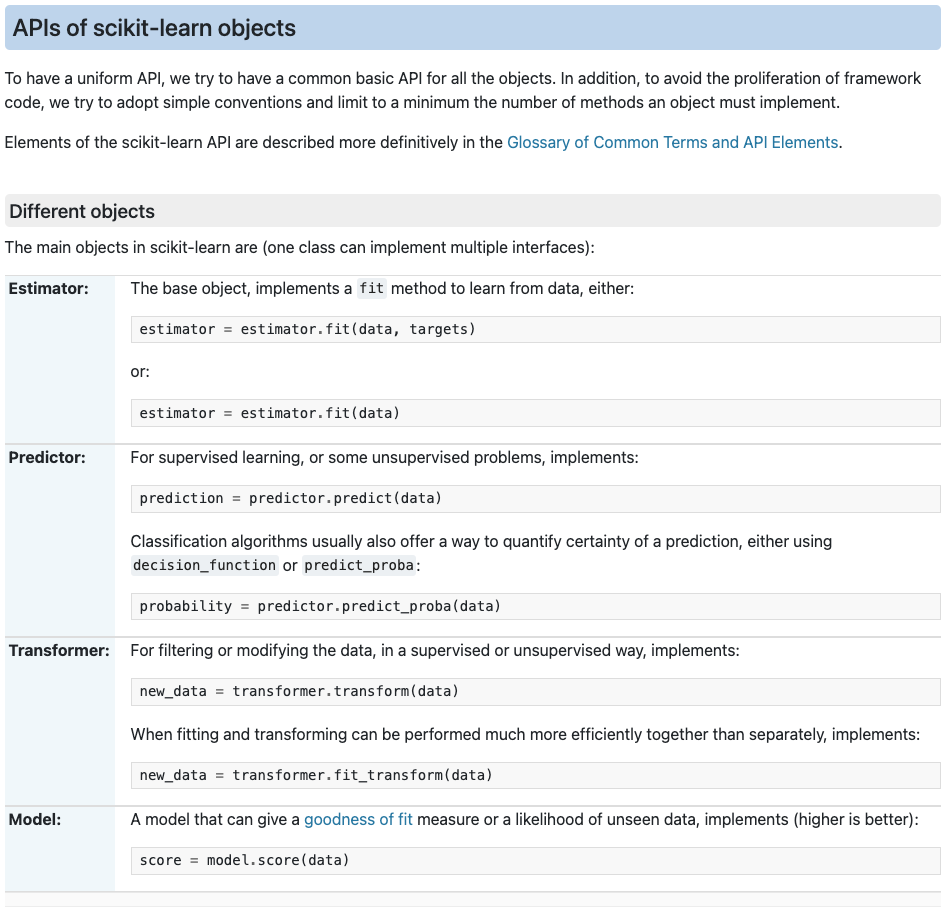
\includegraphics[width=6cm]{data/sklearn_api.png}
            };
        \end{tikzpicture}
        \vfill
    \end{frame}

    \begin{frame}[fragile]{Python: scikit-learn} % Linear regression
        \begin{tikzpicture}
            \node[
                minimum width=\codewidth,
                text width=\codewidth,
                align=left,
                inner sep=0pt,
                anchor=north,
                label={[blue,
                        anchor=north east,
                        font=\ttfamily\fontsize{5}{6}\selectfont,
                        inner sep=0pt,
                        outer sep=0pt,
                        xshift=-3pt,
                        yshift=-3.5pt,
                        text depth=0
                        ]north west:In{[}1{]}:}
            ] (code) at (0, 0) {
                \begin{lstlisting}[style=PythonStyle]
from sklearn.linear_model import LinearRegression

path = '/Users/esten/Downloads/Auto.csv'
df = pd.read_csv(path)

predictors = ['cylinders', 'displacement', 'horsepower',
              'weight', 'acceleration', 'year']
target = 'mpg'

model = LinearRegression()
model.fit(df[predictors], df[target])

# Print model coefficients
print(f'Intercept: {model.intercept_}')
print(f'Coefficients: {model.coef_}')

# Print model residuals
predictions = model.predict(df[predictors])
residuals = df[target] - predictions
print(f'Residuals: {residuals.values[:5]}...')
                \end{lstlisting}
            };

            \node[
                minimum width=\codewidth,
                text width=\codewidth,
                align=left,
                inner sep=0pt,
                anchor=north,
                label={[red,
                        anchor=north east,
                        font=\ttfamily\fontsize{5}{6}\selectfont,
                        inner sep=0pt,
                        outer sep=0pt,
                        xshift=-3pt,
                        yshift=-3.5pt,
                        text depth=0
                        ]north west:Out{[}1{]}:}
            ] (output) at ($ (code.south) - (0, 0.2) $) {
                \begin{lstlisting}[style=PythonOutput]
Intercept: -14.53525048050604
Coefficients: [-3.29859089e-01  7.67843024e-03 -3.91355574e-04 -6.79461791e-03
    8.52732469e-02  7.53367180e-01]
Residuals: [2.91708096 0.92742531 2.46368456 0.46552549 1.71359255]...
                \end{lstlisting}
            };
            \node[] at (4.4, -6.8) {};
            \node[] at (-5.4, -0.1) {};
        \end{tikzpicture}
    \end{frame}

    \begin{frame}[fragile]{Python: scikit-learn} % Support vector regression
        \begin{tikzpicture}
            \node[
                minimum width=\codewidth,
                text width=\codewidth,
                align=left,
                inner sep=0pt,
                anchor=north,
                label={[blue,
                        anchor=north east,
                        font=\ttfamily\fontsize{5}{6}\selectfont,
                        inner sep=0pt,
                        outer sep=0pt,
                        xshift=-3pt,
                        yshift=-3.5pt,
                        text depth=0
                        ]north west:In{[}1{]}:}
            ] (code) at (0, 0) {
                \begin{lstlisting}[style=PythonStyle]
from sklearn.svm import SVR

path = '/Users/esten/Downloads/Auto.csv'
df = pd.read_csv(path)

predictors = ['cylinders', 'displacement', 'horsepower',
              'weight', 'acceleration', 'year']
target = 'mpg'

model = SVR(kernel='linear')
model.fit(df[predictors], df[target])

# Print model coefficients
print(f'Intercept: {model.intercept_}')
print(f'Coefficients: {model.coef_}')

# Print model residuals
predictions = model.predict(df[predictors])
residuals = df[target] - predictions
print(f'Residuals: {residuals.values[:5]}...')
                \end{lstlisting}
            };

            \node[
                minimum width=\codewidth,
                text width=\codewidth,
                align=left,
                inner sep=0pt,
                anchor=north,
                label={[red,
                        anchor=north east,
                        font=\ttfamily\fontsize{5}{6}\selectfont,
                        inner sep=0pt,
                        outer sep=0pt,
                        xshift=-3pt,
                        yshift=-3.5pt,
                        text depth=0
                        ]north west:Out{[}1{]}:}
            ] (output) at ($ (code.south) - (0, 0.2) $) {
                \begin{lstlisting}[style=PythonOutput]
Intercept: [-35.38646279]
Coefficients: [[-1.0526357   0.05910105 -0.03667206 -0.00831565  0.56218046  0.96851648]]
Residuals: [3.0266171  0.62154228 3.10666275 1.34695011 3.07475274]...
                \end{lstlisting}
            };
            \node[] at (4.4, -6.8) {};
            \node[] at (-5.4, -0.1) {};
        \end{tikzpicture}
    \end{frame}

    \def\codewidth{10cm}

    \begin{frame}[fragile]{Coding tips: Separation of concerns} % Spaghetti
        \centering
        \begin{tikzpicture}
            \node[
                minimum width=\codewidth,
                text width=\codewidth,
                align=left,
                inner sep=0pt,
                anchor=north,
                label={[blue,
                        anchor=north east,
                        font=\ttfamily\fontsize{4}{4}\selectfont,
                        inner sep=0pt,
                        outer sep=0pt,
                        xshift=-3pt,
                        yshift=-3.5pt,
                        text depth=0
                        ]north west:In{[}1{]}:}
            ] (code) at (0, 0) {
                \begin{lstlisting}[style=PythonStyle, basicstyle=\ttfamily\fontsize{4}{4}\selectfont]
# Read and clean data
path = '/Users/esten/Downloads/Auto.csv'
df = pd.read_csv(path)

# Split data
train = df.iloc[:int(len(df) * 0.8)]
validation = df.iloc[int(len(df) * 0.8):]

# Define input and output variables
predictors = ['cylinders', 'displacement', 'horsepower',
                'weight', 'acceleration', 'year']
target = 'mpg'

# Define necessary data structures for state
chosen_predictors = []
mses = []

while len(predictors) > 0:
    best_predictor = {'mse': float('inf'), 'predictor': None}

    for predictor in set(predictors) - set(chosen_predictors):
        potential_predictors = chosen_predictors + [predictor]

        # Fit and evaluate model
        model = LinearRegression()
        model.fit(train[potential_predictors], train[target])
        predictions = model.predict(validation[potential_predictors])
        test_mse = np.mean((validation[target] - predictions) ** 2)

        # Compare model with previous best
        if test_mse < best_predictor['mse']:
            best_predictor = {'mse': test_mse, 'predictor': predictor}

    # Update state
    chosen_predictors.append(best_predictor['predictor'])
    mses.append(best_predictor['mse'])
    predictors = [p for p in predictors if p != best_predictor['predictor']]
                \end{lstlisting}
            };
            \node[] at (0, -7.55) {};
        \end{tikzpicture}
    \end{frame}

    \begin{frame}[fragile]{Coding tips: Separation of concerns} % Chunks
        \centering
        \begin{tikzpicture}
            \node[
                minimum width=\codewidth,
                text width=\codewidth,
                align=left,
                inner sep=0pt,
                anchor=north,
                label={[blue,
                        anchor=north east,
                        font=\ttfamily\fontsize{4}{4}\selectfont,
                        inner sep=0pt,
                        outer sep=0pt,
                        xshift=-3pt,
                        yshift=-3.5pt,
                        text depth=0
                        ]north west:In{[}1{]}:}
            ] (code) at (0, 0) {
                \begin{lstlisting}[style=PythonStyle, basicstyle=\ttfamily\fontsize{4}{4}\selectfont]
# Read and clean data
path = '/Users/esten/Downloads/Auto.csv'
df = pd.read_csv(path)

# Split data
train = df.iloc[:int(len(df) * 0.8)]
validation = df.iloc[int(len(df) * 0.8):]

# Define input and output variables
predictors = ['cylinders', 'displacement', 'horsepower',
                'weight', 'acceleration', 'year']
target = 'mpg'

# Define necessary data structures for state
chosen_predictors = []
mses = []

while len(predictors) > 0:
    best_predictor = {'mse': float('inf'), 'predictor': None}

    for predictor in set(predictors) - set(chosen_predictors):
        potential_predictors = chosen_predictors + [predictor]

        # Fit and evaluate model
        model = LinearRegression()
        model.fit(train[potential_predictors], train[target])
        predictions = model.predict(validation[potential_predictors])
        test_mse = np.mean((validation[target] - predictions) ** 2)

        # Compare model with previous best
        if test_mse < best_predictor['mse']:
            best_predictor = {'mse': test_mse, 'predictor': predictor}

    # Update state
    chosen_predictors.append(best_predictor['predictor'])
    mses.append(best_predictor['mse'])
    predictors = [p for p in predictors if p != best_predictor['predictor']]
                \end{lstlisting}
            };
            \node[
                anchor=north west,
                fill=purple,
                inner sep=0pt,
                outer sep=0pt,
                minimum width=\codewidth,
                minimum height=2.78cm,
                opacity=0.2,
                align=right,
            ] (setup) at ($ (code.north west) + (0.01, -0.01) $) {};
            \node[anchor=north east, inner sep=2pt] at (setup.north east) {\textcolor{red}{\tiny{Setup}}};

            \node[
                anchor=north west,
                fill=green,
                inner sep=0pt,
                outer sep=0pt,
                minimum width=\codewidth,
                minimum height=3.478cm,
                opacity=0.2
            ] (selection) at (setup.south west) {};
            \node[anchor=north east, inner sep=2pt] at (selection.north east) {\textcolor{green}{\tiny{Selection}}};

            \node[
                anchor=north west,
                fill=blue,
                inner sep=0pt,
                outer sep=0pt,
                minimum width=\codewidth - 0.8cm,
                minimum height=1cm,
                opacity=0.2
            ] (training) at ($ (selection.north west) + (0.66, -0.98) $) {};
            \node[anchor=north east, inner sep=2pt] at (training.north east) {\textcolor{blue}{\tiny{Modelling}}};

            \node[
                anchor=north west,
                fill=orange,
                inner sep=0pt,
                outer sep=0pt,
                minimum width=\codewidth - 0.48cm,
                minimum height=0.83cm,
                opacity=0.2
            ] (state) at ($ (selection.north west) + (0.34, -2.6) $) {};
            \node[anchor=north east, inner sep=2pt] at (state.north east) {\textcolor{orange}{\tiny{Housekeeping}}};
            \node[] at (0, -7.55) {};
        \end{tikzpicture}
    \end{frame}

    \begin{frame}[fragile]{Coding tips: Separation of concerns} % Proper
        \begin{tikzpicture}
            \node[
                minimum width=\codewidth,
                text width=\codewidth,
                align=left,
                inner sep=0pt,
                anchor=north,
                label={[blue,
                        anchor=north east,
                        font=\ttfamily\fontsize{4}{4}\selectfont,
                        inner sep=0pt,
                        outer sep=0pt,
                        xshift=-3pt,
                        yshift=-3.5pt,
                        text depth=0
                        ]north west:In{[}1{]}:}
            ] (code) at (0, 0) {
                \begin{lstlisting}[style=PythonStyle, basicstyle=\ttfamily\fontsize{4}{4}\selectfont]
# Read and clean data
path = '/Users/esten/Downloads/Auto.csv'
df = pd.read_csv(path)

# Split data
train = df.iloc[:int(len(df) * 0.8)]
validation = df.iloc[int(len(df) * 0.8):]

# Define input and output variables
predictors = ['cylinders', 'displacement', 'horsepower',
                'weight', 'acceleration', 'year']
target = 'mpg'

# Define necessary data structures for state
chosen_predictors = []
mses = []

def fit_and_evaluate_model(model: LinearRegression, train: pd.DataFrame,
                           validation: pd.DataFrame, variables: List[str],
                           target: str):
    """ Fit a given model on a training dataset using a given set of variables
    and return MSE from a validation dataset. """
    model = LinearRegression()
    model.fit(train[potential_predictors], train[target])
    predictions = model.predict(validation[potential_predictors])

    return np.mean((validation[target] - predictions) ** 2)

while len(predictors) > 0:
    best_predictor = {'mse': float('inf'), 'predictor': None}

    for predictor in set(predictors) - set(chosen_predictors):
        potential_predictors = chosen_predictors + [predictor]
        test_mse = fit_and_evaluate_model(LinearRegression(), train, validation,
                                            variables=potential_predictors,
                                            target=target)

        # Compare model with previous best
        if test_mse < best_predictor['mse']:
            best_predictor = {'mse': test_mse, 'predictor': predictor}

    # Update state
    chosen_predictors.append(best_predictor['predictor'])
    mses.append(best_predictor['mse'])
    predictors = [p for p in predictors if p != best_predictor['predictor']]
                \end{lstlisting}
            };
            \node[
                anchor=north west,
                fill=blue,
                inner sep=0pt,
                outer sep=0pt,
                minimum width=\codewidth - 0.14cm,
                minimum height=1.8cm,
                opacity=0.2
            ] (training) at ($ (code.north west) + (0.07, -2.8) $) {};
            \node[anchor=north east, inner sep=2pt] at (training.north east) {\textcolor{blue}{\tiny{Modelling}}};

            \node[
                anchor=north west,
                draw=blue,
                line width=0.5pt,
                inner sep=0pt,
                outer sep=0pt,
                minimum width=\codewidth - 1.37cm,
                minimum height=0.52cm
            ] (training) at ($ (code.north west) + (0.74, -5.49) $) {};

            \node[] at (0, -7.55) {};
        \end{tikzpicture}
    \end{frame}

    \begin{frame}{Regularization: Motivation}
        \centering
        \vfill
        $y \sim \beta_0 + \beta_1 * x_1 + \beta_2 * x_2 + \beta_3 * x_3$
        \vfill
    \end{frame}

    \begin{frame}{Regularization: Motivation}
        \centering
        \vfill
        \begin{tikzpicture}
            \node[draw=black, fill=white] {
                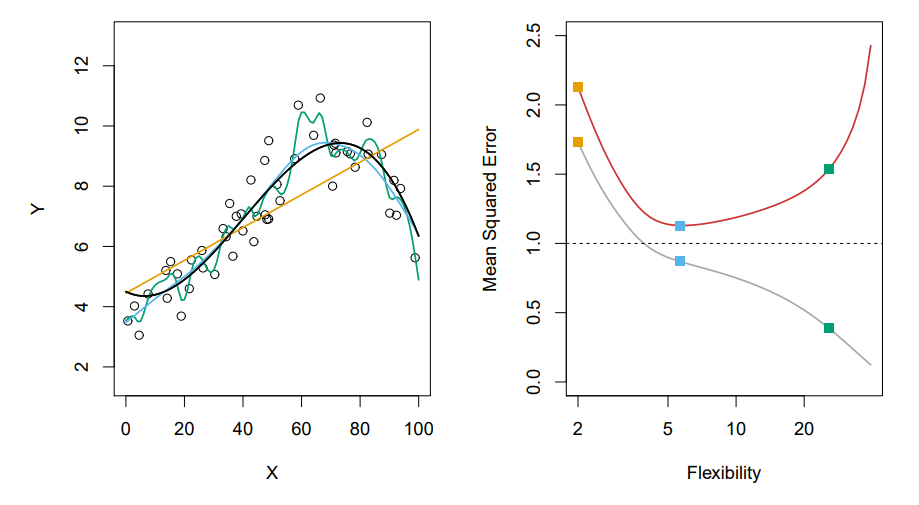
\includegraphics[width=8cm]{data/overfitting.png}
            };
        \end{tikzpicture}
        \vfill
    \end{frame}

    \begin{frame}[fragile]{Regularization: Out-of-sample testing}
        \begin{tikzpicture}
            \node[
                minimum width=\codewidth,
                text width=\codewidth,
                align=left,
                inner sep=0pt,
                anchor=north,
                label={[blue,
                        anchor=north east,
                        font=\ttfamily\fontsize{5}{6}\selectfont,
                        inner sep=0pt,
                        outer sep=0pt,
                        xshift=-3pt,
                        yshift=-3.5pt,
                        text depth=0
                        ]north west:In{[}1{]}:}
            ] (code) at (0, 0) {
                \begin{lstlisting}[style=PythonStyle]
import pandas as pd


df = pd.read_csv('/Users/esten/Downloads/Auto.csv')
train = df.iloc[:int(len(df) * 0.8)]
validation = df.iloc[int(len(df) * 0.8):]

print(f'Using {len(train)} samples for training')
print(f'Using {len(validation)} samples for validation')
                \end{lstlisting}
            };

            \node[
                minimum width=\codewidth,
                text width=\codewidth,
                align=left,
                inner sep=0pt,
                anchor=north,
                label={[red,
                        anchor=north east,
                        font=\ttfamily\fontsize{5}{6}\selectfont,
                        inner sep=0pt,
                        outer sep=0pt,
                        xshift=-3pt,
                        yshift=-3.5pt,
                        text depth=0
                        ]north west:Out{[}1{]}:}
            ] (output) at ($ (code.south) - (0, 0.2) $) {
                \begin{lstlisting}[style=PythonOutput]
Using 317 samples for training
Using 80 samples for validation
                \end{lstlisting}
            };
        \end{tikzpicture}
    \end{frame}

    \begin{frame}{Regularization: Methods}
        \begin{enumerate}
            \item Variable selection
            \begin{enumerate}
                \item[a.] Best subset selection
                \item[b.] Forward stepwise selection
                \item[c.] Backward stepwise selection
            \end{enumerate}
            \item Shrinkage
            \begin{enumerate}
                \item[a.] LASSO
                \item[b.] Ridge Regression
            \end{enumerate}
            \item Dimensionality reduction
            \begin{enumerate}
                \item[a.] Principal Component Regression
                \item[b.] Partial Least Squares
            \end{enumerate}
        \end{enumerate}
    \end{frame}

    \section{Variable selection}

    \begin{frame}{Variable selection: Motivation}
        \centering
        The number of predictors we are using in our model directly impacts model complexity.
    \end{frame}

    \begin{frame}[t]{Variable selection: Outline} % Problem definition
        \underline{Problem}\\
        We have a set of predictors $P=\{x_0, x_1, ...\}$ and a target variable $y$, and we want to find the subset $p \subseteq P$ that yields the best (linear) model for predicting $y$.\\
    \end{frame}

    \begin{frame}[t]{Variable selection: Outline} % Motivation
        \underline{Problem}\\
        We have a set of predictors $P=\{x_0, x_1, ...\}$ and a target variable $y$, and we want to find the subset $p \subseteq P$ that yields the best (linear) model for predicting $y$.\\
        \vspace{0.25cm}
        \underline{Motivation}\\
        \begin{enumerate}
            \item Reduce model complexity (overfitting)
            \item Simplify interpretation
        \end{enumerate}
    \end{frame}

    \def\codewidth{10cm}

    \begin{frame}[t]{Variable selection: Outline} % Variables
        \underline{Problem}\\
        We have a set of predictors $P=\{x_0, x_1, ...\}$ and a target variable $y$, and we want to find the subset $p \subseteq P$ that yields the best (linear) model for predicting $y$.\\
        \vspace{0.25cm}

        \centering
        \begin{tikzpicture}
            \begin{groupplot}[
                group style={
                    group size=3 by 2,
                    horizontal sep=0.5cm
                },
                ticklabel style = {font=\tiny},
                height=3.9cm,
                width=3.9cm
            ]
                \newcommand{\autoplot}[1]{
                    \nextgroupplot[
                        title=\scriptsize{####1},
                        every axis title/.style={at={(0.5,1.15)}}
                    ]
                        \addplot[
                            only marks,
                            mark=*,
                            color=blue,
                            opacity=0.25
                        ] table[
                            col sep=comma,
                            y=mpg,
                            x=####1
                        ] {data/Auto.csv};
                }
                \autoplot{cylinders}
                \autoplot{displacement}
                \autoplot{horsepower}
                \autoplot{weight}
                \autoplot{acceleration}
                \autoplot{year}
            \end{groupplot}

        \end{tikzpicture}
    \end{frame}

    \begin{frame}[t]{Variable selection: Best subset selection} % Implementation
        \underline{Problem}\\
        We have a set of predictors $P=\{x_0, x_1, ...\}$ and a target variable $y$, and we want to find the subset $p \subseteq P$ that yields the best (linear) model for predicting $y$.\\
        \vspace{0.25cm}
        \underline{Solution}\\
        Train models on all subsets $p$ and select the best one.
    \end{frame}

    \begin{frame}[t,fragile]{Variable selection: Best subset selection} % Implementation
        \underline{Problem}\\
        We have a set of predictors $P=\{x_0, x_1, ...\}$ and a target variable $y$, and we want to find the subset $p \subseteq P$ that yields the best (linear) model for predicting $y$.\\
        \vspace{0.25cm}
        \underline{Solution}\\
        \vspace{0.05cm}
        \centering
        \begin{tikzpicture}
            \node[
                minimum width=\codewidth,
                text width=\codewidth,
                align=left,
                inner sep=0pt,
                anchor=north,
                label={[blue,
                        anchor=north east,
                        font=\ttfamily\fontsize{4}{4}\selectfont,
                        inner sep=0pt,
                        outer sep=0pt,
                        xshift=-3pt,
                        yshift=-3.5pt,
                        text depth=0
                        ]north west:In{[}1{]}:}
            ] (code) at (0, 0) {
                \begin{lstlisting}[style=PythonStyle]
import numpy as np

from itertools import chain, combinations
from sklearn.linear_model import LinearRegression

subsets = list(chain.from_iterable(combinations(predictors, r) \
                                    for r in range(len(predictors)+1)))

best = {'mse': float('inf'), 'subset': None}

for subset in subsets:
    if len(subset) == 0:
        continue

    model = LinearRegression()
    model.fit(train[list(subset)], train[target])
    predictions = model.predict(validation[list(subset)])
    mse = np.mean((predictions - validation[target]) ** 2)

    if mse < best['mse']:
        best = {'mse': mse, 'subset': subset}

print(f'MSE: {best["mse"]:.2f}, predictors: {best["subset"]}')
                \end{lstlisting}
            };

            \node[
                minimum width=\codewidth,
                text width=\codewidth,
                align=left,
                inner sep=0pt,
                anchor=north,
                label={[red,
                        anchor=north east,
                        font=\ttfamily\fontsize{4}{4}\selectfont,
                        inner sep=0pt,
                        outer sep=0pt,
                        xshift=-3pt,
                        yshift=-3.5pt,
                        text depth=0
                        ]north west:Out{[}1{]}:}
            ] (output) at ($ (code.south) - (0, 0.1) $) {
                \begin{lstlisting}[style=PythonOutput]
MSE: 29.68, predictors: ('cylinders', 'displacement', 'horsepower', 'weight', 'year')                \end{lstlisting}
            };

        \end{tikzpicture}

    \end{frame}

     \begin{frame}[t]{Variable selection: Best subset selection} % Summary
        \underline{Problem}\\
        We have a set of predictors $P=\{x_0, x_1, ...\}$ and a target variable $y$, and we want to find the subset $p \subseteq P$ that yields the best (linear) model for predicting $y$.\\
        \vspace{0.25cm}
        \underline{Solution}\\
        Train models on all subsets $p$ and select the best one.\\
        \vspace{0.25cm}
        \underline{\textcolor{green}{+} Positives}\\
        Guaranteed to find the optimal solution.\\
        Simple implementation\\
        \vspace{0.25cm}
        \underline{\textcolor{red}{-} Drawbacks}\\
        Need to train many ($2^{|P|}$) models.
     \end{frame}

     \begin{frame}[t]{Variable selection: Best subset selection} % Number of models
        \centering
        \vfill
        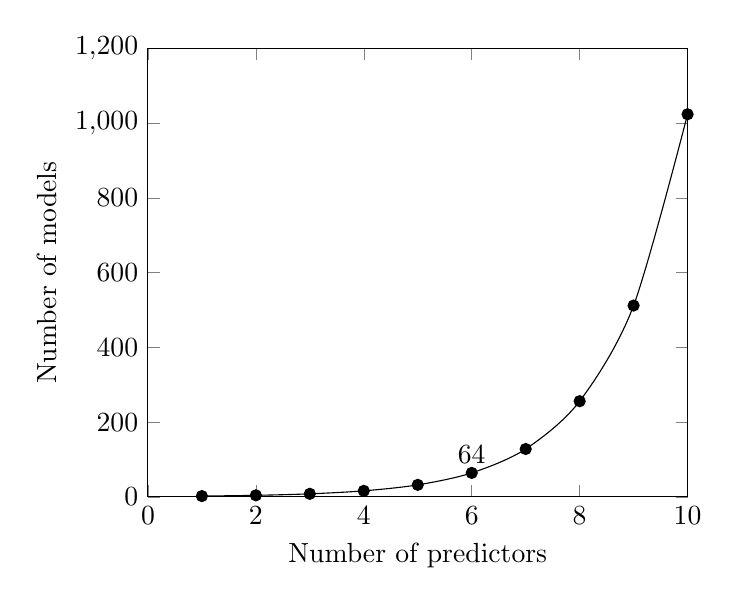
\begin{tikzpicture}
            \begin{axis}[
                smooth,
                xmin=0,
                xmax=10,
                ymin=0,
                ymax=1200,
                xlabel={Number of predictors},
                ylabel={Number of models},
            ]
                \addplot[mark=*] coordinates {
                    (1, 2^1)
                    (2, 2^2)
                    (3, 2^3)
                    (4, 2^4)
                    (5, 2^5)
                    (6, 2^6)
                    (7, 2^7)
                    (8, 2^8)
                    (9, 2^9)
                    (10, 2^10)
                };
                \node[anchor=south] at (axis cs: 6, 2^6) {64};
            \end{axis}
        \end{tikzpicture}
        \vfill
     \end{frame}

     \begin{frame}[t]{Variable selection: Forward stepwise selection} % Intro
        \underline{Problem}\\
        We have a set of predictors $P=\{x_0, x_1, ...\}$ and a target variable $y$, and we want to find the subset $p \subseteq P$ that yields the best (linear) model for predicting $y$.\\
        \vspace{0.25cm}
        \underline{Solution}\\
        Start with no predictors. Iteratively add the predictor that yields the best model until all are included.\\
    \end{frame}

    \begin{frame}[t]{Variable selection: Forward stepwise selection} % Empty model
        \underline{Problem}\\
        We have a set of predictors $P=\{x_0, x_1, ...\}$ and a target variable $y$, and we want to find the subset $p \subseteq P$ that yields the best (linear) model for predicting $y$.\\
        \vspace{0.25cm}
        \underline{Solution}\\
        Start with no predictors. Iteratively add the predictor that yields the best model until all are included.\\
        \vspace{0.25cm}
        \centering

        \def\nodefont{\fontsize{4}{4}\linespread{0.85}\selectfont}
        \def\hsep{1.6}
        \def\vsep{0.75}
        \begin{tikzpicture}
            \node[draw=black, align=center, font=\nodefont] (n00) at (0, 0 * \vsep) {
                $y \sim \mathbbm{1}$\\
                $mse=146.47$
            };

            \node[] at (6.5 * \hsep, 3.3 * \vsep) {};
            \node[] at (-0.32 * \hsep, -3.3 * \vsep) {};
        \end{tikzpicture}
    \end{frame}

    \begin{frame}[t]{Variable selection: Forward stepwise selection} % n-5
        \underline{Problem}\\
        We have a set of predictors $P=\{x_0, x_1, ...\}$ and a target variable $y$, and we want to find the subset $p \subseteq P$ that yields the best (linear) model for predicting $y$.\\
        \vspace{0.25cm}
        \underline{Solution}\\
        Start with no predictors. Iteratively add the predictor that yields the best model until all are included.\\
        \vspace{0.25cm}
        \centering

        \def\nodefont{\fontsize{4}{4}\linespread{0.85}\selectfont}
        \def\hsep{1.6}
        \def\vsep{0.75}
        \begin{tikzpicture}
            \node[draw=black, align=center, font=\nodefont] (n00) at (0, 0 * \vsep) {
                $y \sim \mathbbm{1}$\\
                $mse=146.47$
            };

            \node[draw=black, align=center, font=\nodefont, color=black] (n11) at (\hsep, 2.5 * \vsep) {
                $y \sim cylinders$\\
                $67.96$
            };
            \node[draw=black, align=center, font=\nodefont, color=black] (n12) at (\hsep, 1.5 * \vsep) {
                $y \sim year$\\
                $61.56$
            };
            \node[draw=black, align=center, font=\nodefont, color=black] (n13) at (\hsep, 0.5 * \vsep) {
                $y \sim acceleration$\\
                $119.72$
            };
            \node[draw=black, align=center, font=\nodefont] (n14) at (\hsep, -0.5 * \vsep) {
                $y \sim weight$\\
                $61.18$
            };
            \node[draw=black, align=center, font=\nodefont, color=black] (n15) at (\hsep, -1.5 * \vsep) {
                $y \sim horsepower$\\
                $65.75$
            };
            \node[draw=black, align=center, font=\nodefont, color=black] (n16) at (\hsep, -2.5 * \vsep) {
                $y \sim displacement$\\
                $63.84$
            };


            \draw[black] (n00.east) -- (n11.west);
            \draw[black] (n00.east) -- (n12.west);
            \draw[black] (n00.east) -- (n13.west);
            \draw[black] (n00.east) -- (n14.west);
            \draw[black] (n00.east) -- (n15.west);
            \draw[black] (n00.east) -- (n16.west);

            \node[] at (6.5 * \hsep, 3.3 * \vsep) {};
            \node[] at (-0.32 * \hsep, -3.3 * \vsep) {};

        \end{tikzpicture}
    \end{frame}

    \begin{frame}[t]{Variable selection: Forward stepwise selection} % n-4
        \underline{Problem}\\
        We have a set of predictors $P=\{x_0, x_1, ...\}$ and a target variable $y$, and we want to find the subset $p \subseteq P$ that yields the best (linear) model for predicting $y$.\\
        \vspace{0.25cm}
        \underline{Solution}\\
        Start with no predictors. Iteratively add the predictor that yields the best model until all are included.\\
        \vspace{0.25cm}
        \centering

        \def\nodefont{\fontsize{4}{4}\linespread{0.85}\selectfont}
        \def\hsep{1.6}
        \def\vsep{0.75}
        \begin{tikzpicture}
            \node[draw=black, align=center, font=\nodefont] (n00) at (0, 0 * \vsep) {
                $y \sim \mathbbm{1}$\\
                $mse=146.47$
            };

            \node[draw=gray!25, align=center, font=\nodefont, color=gray!25] (n11) at (\hsep, 2.5 * \vsep) {
                $y \sim cylinders$\\
                $67.96$
            };
            \node[draw=gray!25, align=center, font=\nodefont, color=gray!25] (n12) at (\hsep, 1.5 * \vsep) {
                $y \sim year$\\
                $61.56$
            };
            \node[draw=gray!25, align=center, font=\nodefont, color=gray!25] (n13) at (\hsep, 0.5 * \vsep) {
                $y \sim acceleration$\\
                $119.72$
            };
            \node[draw=black, align=center, font=\nodefont] (n14) at (\hsep, -0.5 * \vsep) {
                $y \sim weight$\\
                $61.18$
            };
            \node[draw=gray!25, align=center, font=\nodefont, color=gray!25] (n15) at (\hsep, -1.5 * \vsep) {
                $y \sim horsepower$\\
                $65.75$
            };
            \node[draw=gray!25, align=center, font=\nodefont, color=gray!25] (n16) at (\hsep, -2.5 * \vsep) {
                $y \sim displacement$\\
                $63.84$
            };

            \node[draw=black, align=center, font=\nodefont, color=black] (n21) at (2 * \hsep, 2.5 * \vsep) {
                $\begin{aligned}
                    y\sim&weight +\\[-0.8em]
                    &cylinders
                \end{aligned}$\\
                $60.02$
            };
            \node[draw=black, align=center, font=\nodefont] (n22) at (2 * \hsep, 1.25 * \vsep) {
                $\begin{aligned}
                    y\sim&weight +\\[-0.8em]
                    &year
                \end{aligned}$\\
                $29.84$
            };
            \node[draw=black, align=center, font=\nodefont, color=black] (n23) at (2 * \hsep, 0 * \vsep) {
                $\begin{aligned}
                    y\sim&weight +\\[-0.8em]
                    &acceleration
                \end{aligned}$\\
                $60.01$
            };
            \node[draw=black, align=center, font=\nodefont, color=black] (n24) at (2 * \hsep, -1.25 * \vsep) {
                $\begin{aligned}
                    y\sim&weight +\\[-0.8em]
                    &horsepower
                \end{aligned}$\\
                $58.59$
            };
            \node[draw=black, align=center, font=\nodefont, color=black] (n25) at (2 * \hsep, -2.5 * \vsep) {
                $\begin{aligned}
                    y\sim&weight +\\[-0.8em]
                    &displacement
                \end{aligned}$\\
                $59.91$
            };

            \draw[gray!25] (n00.east) -- (n11.west);
            \draw[gray!25] (n00.east) -- (n12.west);
            \draw[gray!25] (n00.east) -- (n13.west);
            \draw[black] (n00.east) -- (n14.west);
            \draw[gray!25] (n00.east) -- (n15.west);
            \draw[gray!25] (n00.east) -- (n16.west);

            \draw[black] (n14.east) -- (n21.west);
            \draw[black] (n14.east) -- (n22.west);
            \draw[black] (n14.east) -- (n23.west);
            \draw[black] (n14.east) -- (n24.west);
            \draw[black] (n14.east) -- (n25.west);

            \node[] at (6.5 * \hsep, 3.3 * \vsep) {};
            \node[] at (-0.32 * \hsep, -3.3 * \vsep) {};

        \end{tikzpicture}
    \end{frame}

    \begin{frame}[t]{Variable selection: Forward stepwise selection} % n-3
        \underline{Problem}\\
        We have a set of predictors $P=\{x_0, x_1, ...\}$ and a target variable $y$, and we want to find the subset $p \subseteq P$ that yields the best (linear) model for predicting $y$.\\
        \vspace{0.25cm}
        \underline{Solution}\\
        Start with no predictors. Iteratively add the predictor that yields the best model until all are included.\\
        \vspace{0.25cm}
        \centering

        \def\nodefont{\fontsize{4}{4}\linespread{0.85}\selectfont}
        \def\hsep{1.6}
        \def\vsep{0.75}
        \begin{tikzpicture}
            \node[draw=black, align=center, font=\nodefont] (n00) at (0, 0 * \vsep) {
                $y \sim \mathbbm{1}$\\
                $mse=146.47$
            };

            \node[draw=gray!25, align=center, font=\nodefont, color=gray!25] (n11) at (\hsep, 2.5 * \vsep) {
                $y \sim cylinders$\\
                $67.96$
            };
            \node[draw=gray!25, align=center, font=\nodefont, color=gray!25] (n12) at (\hsep, 1.5 * \vsep) {
                $y \sim year$\\
                $61.56$
            };
            \node[draw=gray!25, align=center, font=\nodefont, color=gray!25] (n13) at (\hsep, 0.5 * \vsep) {
                $y \sim acceleration$\\
                $119.72$
            };
            \node[draw=black, align=center, font=\nodefont] (n14) at (\hsep, -0.5 * \vsep) {
                $y \sim weight$\\
                $61.18$
            };
            \node[draw=gray!25, align=center, font=\nodefont, color=gray!25] (n15) at (\hsep, -1.5 * \vsep) {
                $y \sim horsepower$\\
                $65.75$
            };
            \node[draw=gray!25, align=center, font=\nodefont, color=gray!25] (n16) at (\hsep, -2.5 * \vsep) {
                $y \sim displacement$\\
                $63.84$
            };

            \node[draw=gray!25, align=center, font=\nodefont, color=gray!25] (n21) at (2 * \hsep, 2.5 * \vsep) {
                $\begin{aligned}
                    y\sim&weight +\\[-0.8em]
                    &cylinders
                \end{aligned}$\\
                $60.02$
            };
            \node[draw=black, align=center, font=\nodefont] (n22) at (2 * \hsep, 1.25 * \vsep) {
                $\begin{aligned}
                    y\sim&weight +\\[-0.8em]
                    &year
                \end{aligned}$\\
                $29.84$
            };
            \node[draw=gray!25, align=center, font=\nodefont, color=gray!25] (n23) at (2 * \hsep, 0 * \vsep) {
                $\begin{aligned}
                    y\sim&weight +\\[-0.8em]
                    &acceleration
                \end{aligned}$\\
                $60.01$
            };
            \node[draw=gray!25, align=center, font=\nodefont, color=gray!25] (n24) at (2 * \hsep, -1.25 * \vsep) {
                $\begin{aligned}
                    y\sim&weight +\\[-0.8em]
                    &horsepower
                \end{aligned}$\\
                $58.59$
            };
            \node[draw=gray!25, align=center, font=\nodefont, color=gray!25] (n25) at (2 * \hsep, -2.5 * \vsep) {
                $\begin{aligned}
                    y\sim&weight +\\[-0.8em]
                    &displacement
                \end{aligned}$\\
                $59.91$
            };

            \node[draw=black, align=center, font=\nodefont, color=black] (n31) at (3 * \hsep, 2.25 * \vsep) {
                $\begin{aligned}
                    y\sim&weight +\\[-0.8em]
                    &year +\\[-0.8em]
                    &cylinders
                \end{aligned}$\\
                $29.91$
            };
            \node[draw=black, align=center, font=\nodefont, color=black] (n32) at (3 * \hsep, 0.75 * \vsep) {
                $\begin{aligned}
                    y\sim&weight +\\[-0.8em]
                    &year +\\[-0.8em]
                    &acceleration
                \end{aligned}$\\
                $29.99$
            };
            \node[draw=black, align=center, font=\nodefont] (n33) at (3 * \hsep, -0.75 * \vsep) {
                $\begin{aligned}
                    y\sim&weight +\\[-0.8em]
                    &year +\\[-0.8em]
                    &horsepower
                \end{aligned}$\\
                $29.85$
            };
            \node[draw=black, align=center, font=\nodefont, color=black] (n34) at (3 * \hsep, -2.25 * \vsep) {
                $\begin{aligned}
                    y\sim&weight +\\[-0.8em]
                    &year +\\[-0.8em]
                    &displacement
                \end{aligned}$\\
                $29.96$
            };

            \draw[gray!25] (n00.east) -- (n11.west);
            \draw[gray!25] (n00.east) -- (n12.west);
            \draw[gray!25] (n00.east) -- (n13.west);
            \draw[black] (n00.east) -- (n14.west);
            \draw[gray!25] (n00.east) -- (n15.west);
            \draw[gray!25] (n00.east) -- (n16.west);

            \draw[gray!25] (n14.east) -- (n21.west);
            \draw[black] (n14.east) -- (n22.west);
            \draw[gray!25] (n14.east) -- (n23.west);
            \draw[gray!25] (n14.east) -- (n24.west);
            \draw[gray!25] (n14.east) -- (n25.west);

            \draw[black] (n22.east) -- (n31.west);
            \draw[black] (n22.east) -- (n32.west);
            \draw[black] (n22.east) -- (n33.west);
            \draw[black] (n22.east) -- (n34.west);

            \node[] at (6.5 * \hsep, 3.3 * \vsep) {};
            \node[] at (-0.32 * \hsep, -3.3 * \vsep) {};

        \end{tikzpicture}
    \end{frame}

    \begin{frame}[t]{Variable selection: Forward stepwise selection} % n-2
        \underline{Problem}\\
        We have a set of predictors $P=\{x_0, x_1, ...\}$ and a target variable $y$, and we want to find the subset $p \subseteq P$ that yields the best (linear) model for predicting $y$.\\
        \vspace{0.25cm}
        \underline{Solution}\\
        Start with no predictors. Iteratively add the predictor that yields the best model until all are included.\\
        \vspace{0.25cm}
        \centering

        \def\nodefont{\fontsize{4}{4}\linespread{0.85}\selectfont}
        \def\hsep{1.6}
        \def\vsep{0.75}
        \begin{tikzpicture}
            \node[draw=black, align=center, font=\nodefont] (n00) at (0, 0 * \vsep) {
                $y \sim \mathbbm{1}$\\
                $mse=146.47$
            };

            \node[draw=gray!25, align=center, font=\nodefont, color=gray!25] (n11) at (\hsep, 2.5 * \vsep) {
                $y \sim cylinders$\\
                $67.96$
            };
            \node[draw=gray!25, align=center, font=\nodefont, color=gray!25] (n12) at (\hsep, 1.5 * \vsep) {
                $y \sim year$\\
                $61.56$
            };
            \node[draw=gray!25, align=center, font=\nodefont, color=gray!25] (n13) at (\hsep, 0.5 * \vsep) {
                $y \sim acceleration$\\
                $119.72$
            };
            \node[draw=black, align=center, font=\nodefont] (n14) at (\hsep, -0.5 * \vsep) {
                $y \sim weight$\\
                $61.18$
            };
            \node[draw=gray!25, align=center, font=\nodefont, color=gray!25] (n15) at (\hsep, -1.5 * \vsep) {
                $y \sim horsepower$\\
                $65.75$
            };
            \node[draw=gray!25, align=center, font=\nodefont, color=gray!25] (n16) at (\hsep, -2.5 * \vsep) {
                $y \sim displacement$\\
                $63.84$
            };

            \node[draw=gray!25, align=center, font=\nodefont, color=gray!25] (n21) at (2 * \hsep, 2.5 * \vsep) {
                $\begin{aligned}
                    y\sim&weight +\\[-0.8em]
                    &cylinders
                \end{aligned}$\\
                $60.02$
            };
            \node[draw=black, align=center, font=\nodefont] (n22) at (2 * \hsep, 1.25 * \vsep) {
                $\begin{aligned}
                    y\sim&weight +\\[-0.8em]
                    &year
                \end{aligned}$\\
                $29.84$
            };
            \node[draw=gray!25, align=center, font=\nodefont, color=gray!25] (n23) at (2 * \hsep, 0 * \vsep) {
                $\begin{aligned}
                    y\sim&weight +\\[-0.8em]
                    &acceleration
                \end{aligned}$\\
                $60.01$
            };
            \node[draw=gray!25, align=center, font=\nodefont, color=gray!25] (n24) at (2 * \hsep, -1.25 * \vsep) {
                $\begin{aligned}
                    y\sim&weight +\\[-0.8em]
                    &horsepower
                \end{aligned}$\\
                $58.59$
            };
            \node[draw=gray!25, align=center, font=\nodefont, color=gray!25] (n25) at (2 * \hsep, -2.5 * \vsep) {
                $\begin{aligned}
                    y\sim&weight +\\[-0.8em]
                    &displacement
                \end{aligned}$\\
                $59.91$
            };

            \node[draw=gray!25, align=center, font=\nodefont, color=gray!25] (n31) at (3 * \hsep, 2.25 * \vsep) {
                $\begin{aligned}
                    y\sim&weight +\\[-0.8em]
                    &year +\\[-0.8em]
                    &cylinders
                \end{aligned}$\\
                $29.91$
            };
            \node[draw=gray!25, align=center, font=\nodefont, color=gray!25] (n32) at (3 * \hsep, 0.75 * \vsep) {
                $\begin{aligned}
                    y\sim&weight +\\[-0.8em]
                    &year +\\[-0.8em]
                    &acceleration
                \end{aligned}$\\
                $29.99$
            };
            \node[draw=black, align=center, font=\nodefont] (n33) at (3 * \hsep, -0.75 * \vsep) {
                $\begin{aligned}
                    y\sim&weight +\\[-0.8em]
                    &year +\\[-0.8em]
                    &horsepower
                \end{aligned}$\\
                $29.85$
            };
            \node[draw=gray!25, align=center, font=\nodefont, color=gray!25] (n34) at (3 * \hsep, -2.25 * \vsep) {
                $\begin{aligned}
                    y\sim&weight +\\[-0.8em]
                    &year +\\[-0.8em]
                    &displacement
                \end{aligned}$\\
                $29.96$
            };

            \node[draw=black, align=center, font=\nodefont, color=black] (n41) at (4 * \hsep, 1.75 * \vsep) {
                $\begin{aligned}
                    y\sim&weight +\\[-0.8em]
                    &year +\\[-0.8em]
                    &horsepower +\\[-0.8em]
                    &cylinders
                \end{aligned}$\\
                $29.87$
            };
            \node[draw=black, align=center, font=\nodefont, color=black] (n42) at (4 * \hsep, 0 * \vsep) {
                $\begin{aligned}
                    y\sim&weight +\\[-0.8em]
                    &year +\\[-0.8em]
                    &horsepower +\\[-0.8em]
                    &acceleration
                \end{aligned}$\\
                $30.29$
            };
            \node[draw=black, align=center, font=\nodefont, color=black] (n43) at (4 * \hsep, -1.75 * \vsep) {
                $\begin{aligned}
                    y\sim&weight +\\[-0.8em]
                    &year +\\[-0.8em]
                    &horsepower +\\[-0.8em]
                    &displacement
                \end{aligned}$\\
                $29.95$
            };


            \draw[gray!25] (n00.east) -- (n11.west);
            \draw[gray!25] (n00.east) -- (n12.west);
            \draw[gray!25] (n00.east) -- (n13.west);
            \draw[black] (n00.east) -- (n14.west);
            \draw[gray!25] (n00.east) -- (n15.west);
            \draw[gray!25] (n00.east) -- (n16.west);

            \draw[gray!25] (n14.east) -- (n21.west);
            \draw[black] (n14.east) -- (n22.west);
            \draw[gray!25] (n14.east) -- (n23.west);
            \draw[gray!25] (n14.east) -- (n24.west);
            \draw[gray!25] (n14.east) -- (n25.west);

            \draw[gray!25] (n22.east) -- (n31.west);
            \draw[gray!25] (n22.east) -- (n32.west);
            \draw[black] (n22.east) -- (n33.west);
            \draw[gray!25] (n22.east) -- (n34.west);

            \draw[black] (n33.east) -- (n41.west);
            \draw[black] (n33.east) -- (n42.west);
            \draw[black] (n33.east) -- (n43.west);

            \node[] at (6.5 * \hsep, 3.3 * \vsep) {};
            \node[] at (-0.32 * \hsep, -3.3 * \vsep) {};

        \end{tikzpicture}
    \end{frame}

    \begin{frame}[t]{Variable selection: Forward stepwise selection} % n-1
        \underline{Problem}\\
        We have a set of predictors $P=\{x_0, x_1, ...\}$ and a target variable $y$, and we want to find the subset $p \subseteq P$ that yields the best (linear) model for predicting $y$.\\
        \vspace{0.25cm}
        \underline{Solution}\\
        Start with no predictors. Iteratively add the predictor that yields the best model until all are included.\\
        \vspace{0.25cm}
        \centering

        \def\nodefont{\fontsize{4}{4}\linespread{0.85}\selectfont}
        \def\hsep{1.6}
        \def\vsep{0.75}
        \begin{tikzpicture}
            \node[draw=black, align=center, font=\nodefont] (n00) at (0, 0 * \vsep) {
                $y \sim \mathbbm{1}$\\
                $mse=146.47$
            };

            \node[draw=gray!25, align=center, font=\nodefont, color=gray!25] (n11) at (\hsep, 2.5 * \vsep) {
                $y \sim cylinders$\\
                $67.96$
            };
            \node[draw=gray!25, align=center, font=\nodefont, color=gray!25] (n12) at (\hsep, 1.5 * \vsep) {
                $y \sim year$\\
                $61.56$
            };
            \node[draw=gray!25, align=center, font=\nodefont, color=gray!25] (n13) at (\hsep, 0.5 * \vsep) {
                $y \sim acceleration$\\
                $119.72$
            };
            \node[draw=black, align=center, font=\nodefont] (n14) at (\hsep, -0.5 * \vsep) {
                $y \sim weight$\\
                $61.18$
            };
            \node[draw=gray!25, align=center, font=\nodefont, color=gray!25] (n15) at (\hsep, -1.5 * \vsep) {
                $y \sim horsepower$\\
                $65.75$
            };
            \node[draw=gray!25, align=center, font=\nodefont, color=gray!25] (n16) at (\hsep, -2.5 * \vsep) {
                $y \sim displacement$\\
                $63.84$
            };

            \node[draw=gray!25, align=center, font=\nodefont, color=gray!25] (n21) at (2 * \hsep, 2.5 * \vsep) {
                $\begin{aligned}
                    y\sim&weight +\\[-0.8em]
                    &cylinders
                \end{aligned}$\\
                $60.02$
            };
            \node[draw=black, align=center, font=\nodefont] (n22) at (2 * \hsep, 1.25 * \vsep) {
                $\begin{aligned}
                    y\sim&weight +\\[-0.8em]
                    &year
                \end{aligned}$\\
                $29.84$
            };
            \node[draw=gray!25, align=center, font=\nodefont, color=gray!25] (n23) at (2 * \hsep, 0 * \vsep) {
                $\begin{aligned}
                    y\sim&weight +\\[-0.8em]
                    &acceleration
                \end{aligned}$\\
                $60.01$
            };
            \node[draw=gray!25, align=center, font=\nodefont, color=gray!25] (n24) at (2 * \hsep, -1.25 * \vsep) {
                $\begin{aligned}
                    y\sim&weight +\\[-0.8em]
                    &horsepower
                \end{aligned}$\\
                $58.59$
            };
            \node[draw=gray!25, align=center, font=\nodefont, color=gray!25] (n25) at (2 * \hsep, -2.5 * \vsep) {
                $\begin{aligned}
                    y\sim&weight +\\[-0.8em]
                    &displacement
                \end{aligned}$\\
                $59.91$
            };

            \node[draw=gray!25, align=center, font=\nodefont, color=gray!25] (n31) at (3 * \hsep, 2.25 * \vsep) {
                $\begin{aligned}
                    y\sim&weight +\\[-0.8em]
                    &year +\\[-0.8em]
                    &cylinders
                \end{aligned}$\\
                $29.91$
            };
            \node[draw=gray!25, align=center, font=\nodefont, color=gray!25] (n32) at (3 * \hsep, 0.75 * \vsep) {
                $\begin{aligned}
                    y\sim&weight +\\[-0.8em]
                    &year +\\[-0.8em]
                    &acceleration
                \end{aligned}$\\
                $29.99$
            };
            \node[draw=black, align=center, font=\nodefont] (n33) at (3 * \hsep, -0.75 * \vsep) {
                $\begin{aligned}
                    y\sim&weight +\\[-0.8em]
                    &year +\\[-0.8em]
                    &horsepower
                \end{aligned}$\\
                $29.85$
            };
            \node[draw=gray!25, align=center, font=\nodefont, color=gray!25] (n34) at (3 * \hsep, -2.25 * \vsep) {
                $\begin{aligned}
                    y\sim&weight +\\[-0.8em]
                    &year +\\[-0.8em]
                    &displacement
                \end{aligned}$\\
                $29.96$
            };

            \node[draw=black, align=center, font=\nodefont, color=black] (n41) at (4 * \hsep, 1.75 * \vsep) {
                $\begin{aligned}
                    y\sim&weight +\\[-0.8em]
                    &year +\\[-0.8em]
                    &horsepower +\\[-0.8em]
                    &cylinders
                \end{aligned}$\\
                $29.87$
            };
            \node[draw=gray!25, align=center, font=\nodefont, color=gray!25] (n42) at (4 * \hsep, 0 * \vsep) {
                $\begin{aligned}
                    y\sim&weight +\\[-0.8em]
                    &year +\\[-0.8em]
                    &horsepower +\\[-0.8em]
                    &acceleration
                \end{aligned}$\\
                $30.29$
            };
            \node[draw=gray!25, align=center, font=\nodefont, color=gray!25] (n43) at (4 * \hsep, -1.75 * \vsep) {
                $\begin{aligned}
                    y\sim&weight +\\[-0.8em]
                    &year +\\[-0.8em]
                    &horsepower +\\[-0.8em]
                    &displacement
                \end{aligned}$\\
                $29.95$
            };


            \node[draw=black, align=center, font=\nodefont] (n51) at (5 * \hsep, 1 * \vsep) {
                $\begin{aligned}
                    y\sim&weight +\\[-0.8em]
                    &year +\\[-0.8em]
                    &horsepower +\\[-0.8em]
                    &cylinders +\\[-0.8em]
                    &acceleration
                \end{aligned}$\\
                $29.68$
            };
            \node[draw=black, align=center, font=\nodefont, color=black] (n52) at (5 * \hsep, -1 * \vsep) {
                $\begin{aligned}
                    y\sim&weight +\\[-0.8em]
                    &year +\\[-0.8em]
                    &horsepower +\\[-0.8em]
                    &cylinders +\\[-0.8em]
                    &displacement
                \end{aligned}$\\
                $30.47$
            };


            \draw[gray!25] (n00.east) -- (n11.west);
            \draw[gray!25] (n00.east) -- (n12.west);
            \draw[gray!25] (n00.east) -- (n13.west);
            \draw[black] (n00.east) -- (n14.west);
            \draw[gray!25] (n00.east) -- (n15.west);
            \draw[gray!25] (n00.east) -- (n16.west);

            \draw[gray!25] (n14.east) -- (n21.west);
            \draw[black] (n14.east) -- (n22.west);
            \draw[gray!25] (n14.east) -- (n23.west);
            \draw[gray!25] (n14.east) -- (n24.west);
            \draw[gray!25] (n14.east) -- (n25.west);

            \draw[gray!25] (n22.east) -- (n31.west);
            \draw[gray!25] (n22.east) -- (n32.west);
            \draw[black] (n22.east) -- (n33.west);
            \draw[gray!25] (n22.east) -- (n34.west);

            \draw[black] (n33.east) -- (n41.west);
            \draw[gray!25] (n33.east) -- (n42.west);
            \draw[gray!25] (n33.east) -- (n43.west);

            \draw[black] (n41.east) -- (n51.west);
            \draw[black] (n41.east) -- (n52.west);

            \node[] at (6.5 * \hsep, 3.3 * \vsep) {};
            \node[] at (-0.32 * \hsep, -3.3 * \vsep) {};

        \end{tikzpicture}
    \end{frame}

    \begin{frame}[t]{Variable selection: Forward stepwise selection} % Full model
        \underline{Problem}\\
        We have a set of predictors $P=\{x_0, x_1, ...\}$ and a target variable $y$, and we want to find the subset $p \subseteq P$ that yields the best (linear) model for predicting $y$.\\
        \vspace{0.25cm}
        \underline{Solution}\\
        Start with no predictors. Iteratively add the predictor that yields the best model until all are included.\\
        \vspace{0.25cm}
        \centering

        \def\nodefont{\fontsize{4}{4}\linespread{0.85}\selectfont}
        \def\hsep{1.6}
        \def\vsep{0.75}
        \begin{tikzpicture}
            \node[draw=black, align=center, font=\nodefont] (n00) at (0, 0 * \vsep) {
                $y \sim \mathbbm{1}$\\
                $mse=146.47$
            };

            \node[draw=gray!25, align=center, font=\nodefont, color=gray!25] (n11) at (\hsep, 2.5 * \vsep) {
                $y \sim cylinders$\\
                $67.96$
            };
            \node[draw=gray!25, align=center, font=\nodefont, color=gray!25] (n12) at (\hsep, 1.5 * \vsep) {
                $y \sim year$\\
                $61.56$
            };
            \node[draw=gray!25, align=center, font=\nodefont, color=gray!25] (n13) at (\hsep, 0.5 * \vsep) {
                $y \sim acceleration$\\
                $119.72$
            };
            \node[draw=black, align=center, font=\nodefont] (n14) at (\hsep, -0.5 * \vsep) {
                $y \sim weight$\\
                $61.18$
            };
            \node[draw=gray!25, align=center, font=\nodefont, color=gray!25] (n15) at (\hsep, -1.5 * \vsep) {
                $y \sim horsepower$\\
                $65.75$
            };
            \node[draw=gray!25, align=center, font=\nodefont, color=gray!25] (n16) at (\hsep, -2.5 * \vsep) {
                $y \sim displacement$\\
                $63.84$
            };

            \node[draw=gray!25, align=center, font=\nodefont, color=gray!25] (n21) at (2 * \hsep, 2.5 * \vsep) {
                $\begin{aligned}
                    y\sim&weight +\\[-0.8em]
                    &cylinders
                \end{aligned}$\\
                $60.02$
            };
            \node[draw=black, align=center, font=\nodefont] (n22) at (2 * \hsep, 1.25 * \vsep) {
                $\begin{aligned}
                    y\sim&weight +\\[-0.8em]
                    &year
                \end{aligned}$\\
                $29.84$
            };
            \node[draw=gray!25, align=center, font=\nodefont, color=gray!25] (n23) at (2 * \hsep, 0 * \vsep) {
                $\begin{aligned}
                    y\sim&weight +\\[-0.8em]
                    &acceleration
                \end{aligned}$\\
                $60.01$
            };
            \node[draw=gray!25, align=center, font=\nodefont, color=gray!25] (n24) at (2 * \hsep, -1.25 * \vsep) {
                $\begin{aligned}
                    y\sim&weight +\\[-0.8em]
                    &horsepower
                \end{aligned}$\\
                $58.59$
            };
            \node[draw=gray!25, align=center, font=\nodefont, color=gray!25] (n25) at (2 * \hsep, -2.5 * \vsep) {
                $\begin{aligned}
                    y\sim&weight +\\[-0.8em]
                    &displacement
                \end{aligned}$\\
                $59.91$
            };

            \node[draw=gray!25, align=center, font=\nodefont, color=gray!25] (n31) at (3 * \hsep, 2.25 * \vsep) {
                $\begin{aligned}
                    y\sim&weight +\\[-0.8em]
                    &year +\\[-0.8em]
                    &cylinders
                \end{aligned}$\\
                $29.91$
            };
            \node[draw=gray!25, align=center, font=\nodefont, color=gray!25] (n32) at (3 * \hsep, 0.75 * \vsep) {
                $\begin{aligned}
                    y\sim&weight +\\[-0.8em]
                    &year +\\[-0.8em]
                    &acceleration
                \end{aligned}$\\
                $29.99$
            };
            \node[draw=black, align=center, font=\nodefont] (n33) at (3 * \hsep, -0.75 * \vsep) {
                $\begin{aligned}
                    y\sim&weight +\\[-0.8em]
                    &year +\\[-0.8em]
                    &horsepower
                \end{aligned}$\\
                $29.85$
            };
            \node[draw=gray!25, align=center, font=\nodefont, color=gray!25] (n34) at (3 * \hsep, -2.25 * \vsep) {
                $\begin{aligned}
                    y\sim&weight +\\[-0.8em]
                    &year +\\[-0.8em]
                    &displacement
                \end{aligned}$\\
                $29.96$
            };

            \node[draw=black, align=center, font=\nodefont, color=black] (n41) at (4 * \hsep, 1.75 * \vsep) {
                $\begin{aligned}
                    y\sim&weight +\\[-0.8em]
                    &year +\\[-0.8em]
                    &horsepower +\\[-0.8em]
                    &cylinders
                \end{aligned}$\\
                $29.87$
            };
            \node[draw=gray!25, align=center, font=\nodefont, color=gray!25] (n42) at (4 * \hsep, 0 * \vsep) {
                $\begin{aligned}
                    y\sim&weight +\\[-0.8em]
                    &year +\\[-0.8em]
                    &horsepower +\\[-0.8em]
                    &acceleration
                \end{aligned}$\\
                $30.29$
            };
            \node[draw=gray!25, align=center, font=\nodefont, color=gray!25] (n43) at (4 * \hsep, -1.75 * \vsep) {
                $\begin{aligned}
                    y\sim&weight +\\[-0.8em]
                    &year +\\[-0.8em]
                    &horsepower +\\[-0.8em]
                    &displacement
                \end{aligned}$\\
                $29.95$
            };


            \node[draw=black, align=center, font=\nodefont] (n51) at (5 * \hsep, 1 * \vsep) {
                $\begin{aligned}
                    y\sim&weight +\\[-0.8em]
                    &year +\\[-0.8em]
                    &horsepower +\\[-0.8em]
                    &cylinders +\\[-0.8em]
                    &acceleration
                \end{aligned}$\\
                $29.68$
            };
            \node[draw=gray!25, align=center, font=\nodefont, color=gray!25] (n52) at (5 * \hsep, -1 * \vsep) {
                $\begin{aligned}
                    y\sim&weight +\\[-0.8em]
                    &year +\\[-0.8em]
                    &horsepower +\\[-0.8em]
                    &cylinders +\\[-0.8em]
                    &displacement
                \end{aligned}$\\
                $30.47$
            };

            \node[draw=black, align=center, font=\nodefont] (n61) at (6 * \hsep, 0 * \vsep) {
                $\begin{aligned}
                    y\sim&weight +\\[-0.8em]
                    &year +\\[-0.8em]
                    &horsepower +\\[-0.8em]
                    &cylinders +\\[-0.8em]
                    &acceleration +\\[-0.8em]
                    &displacement
                \end{aligned}$\\
                $30.29$
            };

            \draw[gray!25] (n00.east) -- (n11.west);
            \draw[gray!25] (n00.east) -- (n12.west);
            \draw[gray!25] (n00.east) -- (n13.west);
            \draw[black] (n00.east) -- (n14.west);
            \draw[gray!25] (n00.east) -- (n15.west);
            \draw[gray!25] (n00.east) -- (n16.west);

            \draw[gray!25] (n14.east) -- (n21.west);
            \draw[black] (n14.east) -- (n22.west);
            \draw[gray!25] (n14.east) -- (n23.west);
            \draw[gray!25] (n14.east) -- (n24.west);
            \draw[gray!25] (n14.east) -- (n25.west);

            \draw[gray!25] (n22.east) -- (n31.west);
            \draw[gray!25] (n22.east) -- (n32.west);
            \draw[black] (n22.east) -- (n33.west);
            \draw[gray!25] (n22.east) -- (n34.west);

            \draw[black] (n33.east) -- (n41.west);
            \draw[gray!25] (n33.east) -- (n42.west);
            \draw[gray!25] (n33.east) -- (n43.west);

            \draw[black] (n41.east) -- (n51.west);
            \draw[gray!25] (n41.east) -- (n52.west);

            \draw[black] (n51.east) -- (n61.west);

            \node[] at (6.5 * \hsep, 3.3 * \vsep) {};
            \node[] at (-0.32 * \hsep, -3.3 * \vsep) {};

        \end{tikzpicture}
    \end{frame}

    \begin{frame}{Variable selection: Forward stepwise selection} % Loss curves
        \centering
        \vfill
        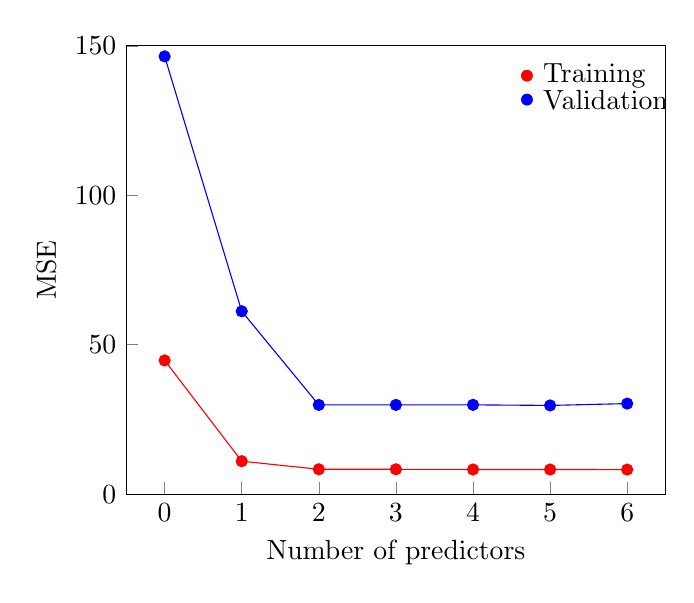
\begin{tikzpicture}
            \begin{axis}[
                xmin=-0.5,
                xmax=6.5,
                ymin=0,
                ymax=150,
                ytick pos=left,
                xtick pos=bottom,
                ylabel=MSE,
                xlabel=Number of predictors
            ]
                \addplot[red,mark=*] coordinates {
                    (0, 44.74)
                    (1, 11.02)
                    (2, 8.31)
                    (3, 8.31)
                    (4, 8.25)
                    (5, 8.24)
                    (6, 8.21)
                };
                \addplot[blue,mark=*] coordinates {
                    (0, 146.47)
                    (1, 61.18)
                    (2, 29.84)
                    (3, 29.85)
                    (4, 29.87)
                    (5, 29.68)
                    (6, 30.29)
                };

                \node[
                    circle,
                    fill=red,
                    minimum size=4.3pt,
                    inner sep=0pt,
                    label=right:Training
                ] at (axis cs: 4.7, 140) {};
                \node[
                    circle,
                    fill=blue,
                    minimum size=4.3pt,
                    inner sep=0pt,
                    label=right:Validation
                ] at (axis cs: 4.7, 132) {};
            \end{axis}
        \end{tikzpicture}
        \vfill
    \end{frame}

    \begin{frame}{Variable selection: Forward stepwise selection} % Optimal models
        \centering
        \vfill
        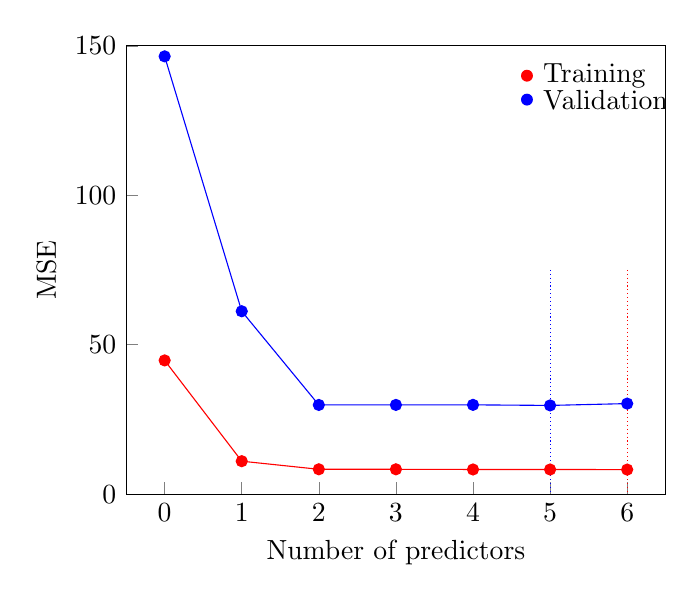
\begin{tikzpicture}
            \begin{axis}[
                xmin=-0.5,
                xmax=6.5,
                ymin=0,
                ymax=150,
                ytick pos=left,
                xtick pos=bottom,
                ylabel=MSE,
                xlabel=Number of predictors
            ]
                \addplot[red,mark=*] coordinates {
                    (0, 44.74)
                    (1, 11.02)
                    (2, 8.31)
                    (3, 8.31)
                    (4, 8.25)
                    (5, 8.24)
                    (6, 8.21)
                };
                \addplot[blue,mark=*] coordinates {
                    (0, 146.47)
                    (1, 61.18)
                    (2, 29.84)
                    (3, 29.85)
                    (4, 29.87)
                    (5, 29.68)
                    (6, 30.29)
                };

                \node[
                    circle,
                    fill=red,
                    minimum size=4.3pt,
                    inner sep=0pt,
                    label=right:Training
                ] at (axis cs: 4.7, 140) {};
                \node[
                    circle,
                    fill=blue,
                    minimum size=4.3pt,
                    inner sep=0pt,
                    label=right:Validation
                ] at (axis cs: 4.7, 132) {};

                \draw[blue, densely dotted] (axis cs: 5, 75) -- (axis cs: 5, 0);
                \draw[red, densely dotted] (axis cs: 6, 75) -- (axis cs: 6, 0);
            \end{axis}
        \end{tikzpicture}
        \vfill
    \end{frame}

    \begin{frame}[t,fragile]{Variable selection: Forward stepwise selection} %Implementation
        \underline{Problem}\\
        We have a set of predictors $P=\{x_0, x_1, ...\}$ and a target variable $y$, and we want to find the subset $p \subseteq P$ that yields the best (linear) model for predicting $y$.\\
        \vspace{0.25cm}
        \underline{Solution}\\
        \begin{tikzpicture}
            \node[
                minimum width=\codewidth,
                text width=\codewidth,
                align=left,
                inner sep=0pt,
                anchor=north,
                label={[blue,
                        anchor=north east,
                        font=\ttfamily\fontsize{4}{4}\selectfont,
                        inner sep=0pt,
                        outer sep=0pt,
                        xshift=-3pt,
                        yshift=-3.5pt,
                        text depth=0
                        ]north west:In{[}1{]}:}
            ] (code) at (0, 0) {
                \begin{lstlisting}[style=PythonStyle, basicstyle=\ttfamily\fontsize{4}{4}\selectfont]
def fit_and_evaluate(train: pd.DataFrame, validation: pd.DataFrame,
                     predictors: List[str], target: str):
   model = LinearRegression()
   model.fit(train[predictors], train[target])

   train_predictions = model.predict(train[predictors])
   validation_predictions = model.predict(validation[predictors])

   return np.mean((train_predictions - train[target]) ** 2), \
          np.mean((validation_predictions - validation[target]) ** 2)

predictors = ['cylinders', 'displacement', 'horsepower', 'weight', 'acceleration', 'year']
target = 'mpg'

train['intercept'] = 1
validation['intercept'] = 1
train_mse, validation_mse = fit_and_evaluate(train, validation,
                                            predictors=['intercept'],
                                            target=target)
print(f'[]: {validation_mse:.2f} ({train_mse:.2f})')

chosen_predictors = []

while len(chosen_predictors) < len(predictors):
   best_predictor = {'train_mse': None, 'validation_mse': float('inf'),
                     'predictor': None}

   for predictor in set(predictors) - set(chosen_predictors):
       train_mse, validation_mse = fit_and_evaluate(train, validation,
                                   predictors=chosen_predictors + [predictor],
                                   target=target)

       if validation_mse < best_predictor['validation_mse']:
           best_predictor = {'train_mse': train_mse, 'validation_mse': validation_mse, 'predictor': predictor}

   chosen_predictors.append(best_predictor['predictor'])

   print(f'{chosen_predictors}: {best_predictor["validation_mse"]:.2f} ({best_predictor["train_mse"]:.2f})')
                \end{lstlisting}
            };
        \end{tikzpicture}
    \end{frame}

    \begin{frame}[t]{Variable selection: Forward stepwise selection} % Summary
        \underline{Problem}\\
        We have a set of predictors $P=\{x_0, x_1, ...\}$ and a target variable $y$, and we want to find the subset $p \subseteq P$ that yields the best (linear) model for predicting $y$.\\
        \vspace{0.25cm}
        \underline{Solution}\\
        Start with no predictors. Iteratively add the predictor that yields the best model until all are included.\\
        \vspace{0.25cm}
        \underline{\textcolor{green}{+} Positives}\\
        Need to train fewer models.\\
        \vspace{0.25cm}
        \underline{\textcolor{red}{-} Drawbacks}\\
        Not guaranteed to find the optimal solution.\\
     \end{frame}

    \begin{frame}[t]{Variable selection: Backward stepwise selection}
        \underline{Problem}\\
        We have a set of predictors $P=\{x_0, x_1, ...\}$ and a target variable $y$, and we want to find the subset $p \subseteq P$ that yields the best (linear) model for predicting $y$.\\
        \vspace{0.25cm}
        \underline{Solution}\\
        Start with all predictors. Iteratively remove the predictor that yields the best model until all you have none left.\\
    \end{frame}

    \begin{frame}[t]{Variable selection: Backward stepwise selection}
        \underline{Problem}\\
        We have a set of predictors $P=\{x_0, x_1, ...\}$ and a target variable $y$, and we want to find the subset $p \subseteq P$ that yields the best (linear) model for predicting $y$.\\
        \vspace{0.25cm}
        \underline{Solution}\\
        Start with all predictors. Iteratively remove the predictor that yields the best model until all you have none left.\\
        \vspace{0.25cm}
        \underline{\textcolor{green}{+} Positives}\\
        Need to train fewer models.\\
        \vspace{0.25cm}
        \underline{\textcolor{red}{-} Drawbacks}\\
        Not guaranteed to find the optimal solution.\\
    \end{frame}

    \section{Shrinkage}

    \def\codewidth{5.2cm}

    \begin{frame}[fragile]{Shrinkage: Outline} % Formula
        \centering
        \vfill
        \begin{tikzpicture}
            \node[] at (2.1, -3.5) {
                $y \sim \beta_0 + $\textcolor{red}{$\beta_1$}$x_1 + $\textcolor{red}{$\beta_2$}$x_2 + $\textcolor{red}{$\beta_3$}$x_3 + $\textcolor{red}{$\beta_4$}$x_4 + $\textcolor{red}{$\beta_5$}$x_5 + $\textcolor{red}{$\beta_6$}$x_6$
            };
            \node[] at (0, 2) {};
            \node[] at (0, -4) {};
        \end{tikzpicture}\\
        \vfill
    \end{frame}

    \begin{frame}[fragile]{Shrinkage: Outline} % Coefficients with formula
        \centering
        \vfill
        \begin{tikzpicture}
            \node[
                minimum width=\codewidth,
                text width=\codewidth,
                align=left,
                inner sep=0pt,
                anchor=north west,
                label={[red,
                        anchor=north east,
                        font=\ttfamily\fontsize{5}{6}\selectfont,
                        inner sep=0pt,
                        outer sep=0pt,
                        xshift=-3pt,
                        yshift=-3.5pt,
                        text depth=0
                        ]north west:Out{[}1{]}:}
            ] (pythonout) at (0, 0) {
                \begin{lstlisting}[style=PythonOutput]
coef  std err  P>|t|  [0.025 0.975]
-----------------------------------------------
Intercept    -14.5353 4.764 0.002 -23.90 -5.16
cylinders    -0.3299  0.332 0.321  -0.98  0.32
displacement  0.0077  0.007 0.297  -0.00  0.02
horsepower   -0.0004  0.014 0.977  -0.02  0.02
weight       -0.0068  0.001 0.000  -0.00 -0.00
acceleration  0.0853  0.102 0.404  -0.11  0.28
year          0.7534  0.053 0.000   0.65  0.85
===============================================
                \end{lstlisting}
            };
            \node[] at (2.1, -3.5) {
                $y \sim \beta_0 + $\textcolor{red}{$\beta_1$}$x_1 + $\textcolor{red}{$\beta_2$}$x_2 + $\textcolor{red}{$\beta_3$}$x_3 + $\textcolor{red}{$\beta_4$}$x_4 + $\textcolor{red}{$\beta_5$}$x_5 + $\textcolor{red}{$\beta_6$}$x_6$
            };
            \node[] at (0, 2) {};
            \node[] at (0, -4) {};
        \end{tikzpicture}\\
        \vfill
    \end{frame}

    \begin{frame}{Shrinkage: Outline} % Bias variance decomposition
        \centering
        \vfill
        $mse = bias^2 + variance + irreducible\ error$
        \vfill
    \end{frame}

    \begin{frame}{Shrinkage: Outline} % ISL plot
        \centering
        \vfill
        \begin{tikzpicture}
            \node[draw=black, fill=white] {
                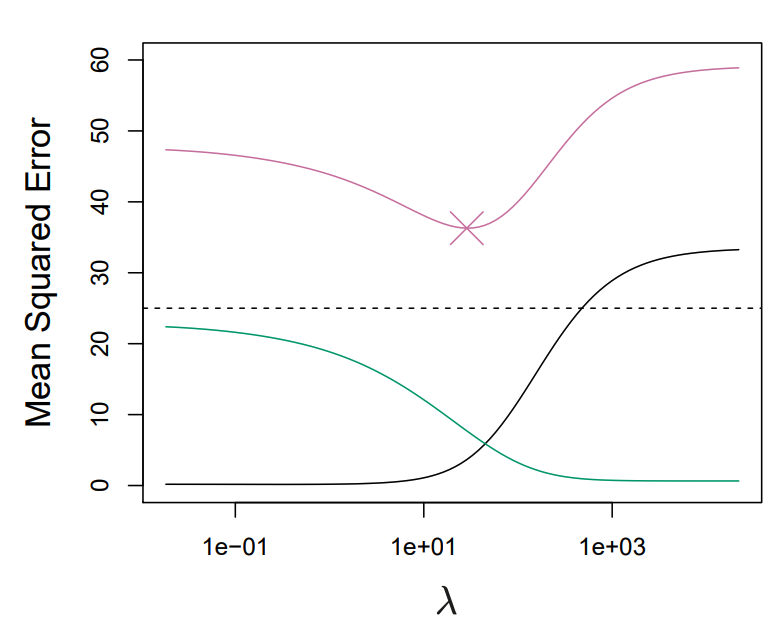
\includegraphics[width=8cm]{data/bias_variance_decomp.png}
            };
        \end{tikzpicture}
        \vfill
    \end{frame}

    \begin{frame}{Shrinkage: Outline} % Salary general model
        \centering
        \vfill
        \begin{tikzpicture}
            \node[] at (0, 0) {
                $salary \sim \beta_0 + \beta_1 * age$
            };
            \node[] at (-6, -2) {};
            \node[] at (6, 1) {};
        \end{tikzpicture}
        \vfill
    \end{frame}

    \begin{frame}{Shrinkage: Outline} % Salary actual models
        \centering
        \vfill
        \begin{tikzpicture}
            \node[] at (0, 0) {
                $salary \sim \beta_0 + \beta_1 * age$
            };

            \node[] at (3, -1) {
                $salary \sim 6000000 + 0 * age$
            };

            \node[] at (-3, -1) {
                $salary \sim 3000000 + 10000 * age$
            };
            \node[] at (-6, -2) {};
            \node[] at (6, 1) {};
        \end{tikzpicture}
        \vfill
    \end{frame}

    \begin{frame}{Shrinkage: Ridge regression} % MSE
        \centering
        \vfill
        \begin{tikzpicture}
            \node[inner sep=0pt] (loss) at (0, 0) {
                $= \sum\limits_{i=0}^n \left( y_i - \sum\limits_{j=0}^p \beta_j x_{ij} \right)^2$
            };
            \node[anchor=east, inner sep=0pt] at (loss.west) {
                $loss_{mse}$
            };

            \node[] at (-2.5, -2) {};
            \node[] at (3.3, 1) {};
        \end{tikzpicture}
        \vfill
    \end{frame}

    \begin{frame}{Shrinkage: Ridge regression} % Ridge loss
        \centering
        \vfill
        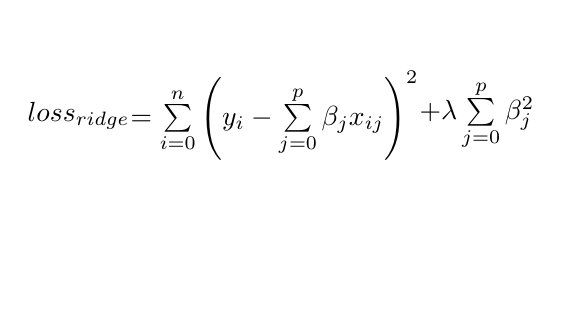
\begin{tikzpicture}
            \node[inner sep=0pt] (loss) at (0, 0) {
                $= \sum\limits_{i=0}^n \left( y_i - \sum\limits_{j=0}^p \beta_j x_{ij} \right)^2$
            };
            \node[anchor=west, inner sep=0pt] (ridge) at (loss.east) {
                $ + \lambda \sum\limits_{j=0}^p \beta_j^2$
            };
            \node[anchor=east, inner sep=0pt] at (loss.west) {
                $loss_{ridge}$
            };

            \node[] at (-2.5, -2) {};
            \node[] at (3.3, 1) {};
        \end{tikzpicture}
        \vfill
    \end{frame}

    \begin{frame}{Shrinkage: Ridge regression} % Ridge interpretation
        \centering
        \vfill
        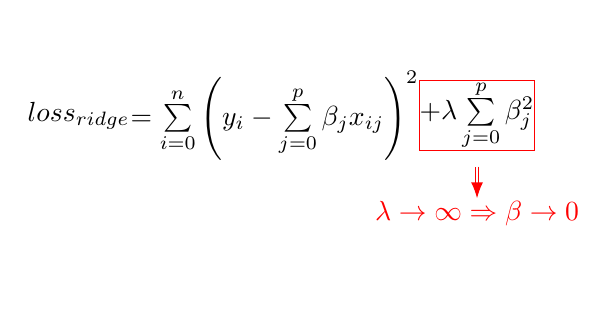
\begin{tikzpicture}
            \node[inner sep=0pt] (loss) at (0, 0) {
                $= \sum\limits_{i=0}^n \left( y_i - \sum\limits_{j=0}^p \beta_j x_{ij} \right)^2$
            };
            \node[anchor=west, inner sep=0pt, draw=red] (ridge) at (loss.east) {
                $ + \lambda \sum\limits_{j=0}^p \beta_j^2$
            };
            \node[anchor=east, inner sep=0pt] at (loss.west) {
                $loss_{ridge}$
            };
            \draw[double, -Latex, red] ($ (ridge.south) - (0, 0.2) $) -- ($ (ridge.south) - (0, 0.6) $);
            \node[red] at ($ (ridge.south) - (0, 0.8) $) {
                $\lambda \to \infty \Rightarrow \beta \to 0$
            };

            \node[] at (-2.5, -2) {};
            \node[] at (3.3, 1) {};
        \end{tikzpicture}
        \vfill
    \end{frame}

    \begin{frame}{Shrinkage} % Ridge coefficients
        \centering
        \vfill
        \begin{tikzpicture}
            \node[draw=black, fill=white] {
                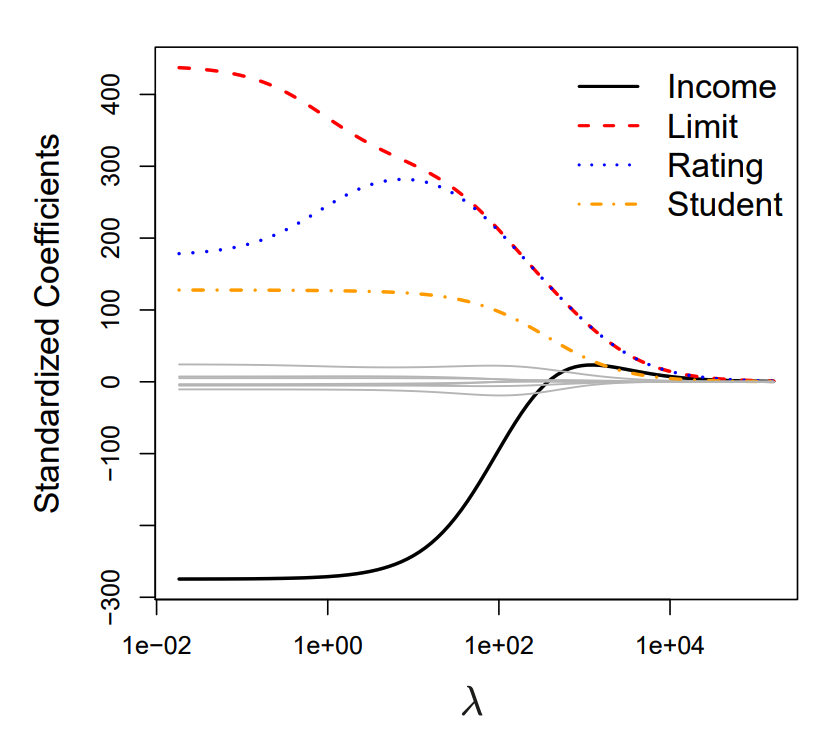
\includegraphics[width=8cm]{data/ridge_coefs.png}
            };
        \end{tikzpicture}
        \vfill
    \end{frame}

    \begin{frame}{Shrinkage: Ridge regression} % Ridge loss for scaling
        \centering
        \vfill
        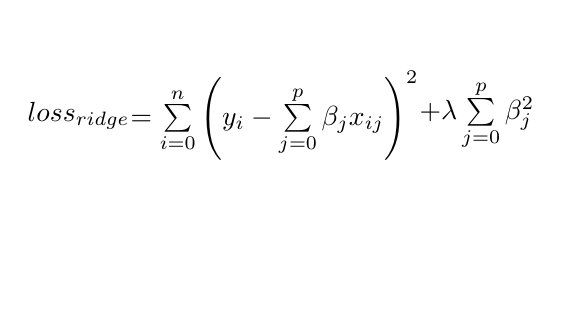
\begin{tikzpicture}
            \node[inner sep=0pt] (loss) at (0, 0) {
                $= \sum\limits_{i=0}^n \left( y_i - \sum\limits_{j=0}^p \beta_j x_{ij} \right)^2$
            };
            \node[anchor=west, inner sep=0pt] (ridge) at (loss.east) {
                $ + \lambda \sum\limits_{j=0}^p \beta_j^2$
            };
            \node[anchor=east, inner sep=0pt] at (loss.west) {
                $loss_{ridge}$
            };

            \node[] at (-2.5, -2) {};
            \node[] at (3.3, 1) {};
        \end{tikzpicture}
        \vfill
    \end{frame}

    \begin{frame}{Shrinkage: Feature standardization} % Variables
        \centering
        \vfill
        \begin{tikzpicture}
            \begin{axis}[
                width=8cm,
                height=8cm,
                xlabel=Acceleration,
                ylabel=Weight
            ]
                \addplot[only marks, blue!50, opacity=0.5] table [col sep=comma, x=acceleration, y=weight] {data/Auto.csv};
            \end{axis}
        \end{tikzpicture}
        \vfill
    \end{frame}

    \def\codewidth{8cm}

    \begin{frame}[fragile]{Shrinkage: Feature standardization} % Name
        \vfill
        \centering
        \begin{tikzpicture}
            \node[] at (0, 0) {\underline{\textbf{z-score standardization}}};
            \node[] at (4.5, -7.5) {};
            \node[] at (-5, 0.5) {};
        \end{tikzpicture}
        \vfill
    \end{frame}

    \begin{frame}[fragile]{Shrinkage: Feature standardization} % Formula
        \vfill
        \centering
        \begin{tikzpicture}
            \node[] at (0, 0) {\underline{\textbf{z-score standardization}}};

            \node[] at (0, -0.7) {
                $\mathbf{x} = \frac{\mathbf{x} - \mu_x}{\sigma_x^2}$
            };
            \node[] at (4.5, -7.5) {};
            \node[] at (-5, 0.5) {};
        \end{tikzpicture}
        \vfill
    \end{frame}

    \begin{frame}[fragile]{Shrinkage: Feature standardization} % Code
        \vfill
        \centering
        \begin{tikzpicture}
            \node[] at (0, 0) {\underline{\textbf{z-score standardization}}};

            \node[] at (0, -0.7) {
                $\mathbf{x} = \frac{\mathbf{x} - \mu_x}{\sigma_x^2}$
            };

            \node[
                minimum width=\codewidth,
                text width=\codewidth,
                align=left,
                inner sep=0pt,
                outer sep=0pt,
                draw=black,
                label={[blue,
                        anchor=north east,
                        font=\ttfamily\fontsize{5}{6}\selectfont,
                        inner sep=0pt,
                        outer sep=0pt,
                        xshift=-3pt,
                        yshift=-3pt
                       ]north west:In{[}1{]}:},
            ] (pythoncode) at (0, -3) {
                \begin{lstlisting}[style=PythonStyle, linewidth=\codewidth]
for col in predictors:
    print(f'{col}: {np.mean(df[col]):.2f} ({np.std(df[col]):.2f})')

# z-score standardization
for col in predictors:
    df[col] = (df[col] - np.mean(df[col])) / np.std(df[col])

for col in predictors:
    print(f'{col} after: {np.mean(df[col]):.2f} ({np.std(df[col]):.2f})')
                \end{lstlisting}
            };
            \node[] at (4.5, -7.5) {};
            \node[] at (-5, 0.5) {};
        \end{tikzpicture}
        \vfill
    \end{frame}

    \begin{frame}[fragile]{Shrinkage: Feature standardization} % Result
        \vfill
        \centering
        \begin{tikzpicture}
            \node[] at (0, 0) {\underline{\textbf{z-score standardization}}};

            \node[] at (0, -0.7) {
                $\mathbf{x} = \frac{\mathbf{x} - \mu_x}{\sigma_x^2}$
            };

            \node[
                minimum width=\codewidth,
                text width=\codewidth,
                align=left,
                inner sep=0pt,
                outer sep=0pt,
                draw=black,
                label={[blue,
                        anchor=north east,
                        font=\ttfamily\fontsize{5}{6}\selectfont,
                        inner sep=0pt,
                        outer sep=0pt,
                        xshift=-3pt,
                        yshift=-3pt
                       ]north west:In{[}1{]}:},
            ] (pythoncode) at (0, -3) {
                \begin{lstlisting}[style=PythonStyle, linewidth=\codewidth]
for col in predictors:
    print(f'{col}: {np.mean(df[col]):.2f} ({np.std(df[col]):.2f})')

# z-score standardization
for col in predictors:
    df[col] = (df[col] - np.mean(df[col])) / np.std(df[col])

for col in predictors:
    print(f'{col} after: {np.mean(df[col]):.2f} ({np.std(df[col]):.2f})')
                \end{lstlisting}
            };

            \node[
                minimum width=\codewidth,
                text width=\codewidth,
                align=left,
                inner sep=0pt,
                label={[red,
                        anchor=north east,
                        font=\ttfamily\fontsize{5}{6}\selectfont,
                        inner sep=0pt,
                        outer sep=0pt,
                        xshift=-3pt,
                        yshift=-3.5pt,
                        text depth=0
                        ]north west:Out{[}1{]}:}
            ] (pythonout) at (0, -6) {
                \begin{lstlisting}[style=PythonOutput]
cylinders: 5.47 (1.70)
displacement: 194.41 (104.51)
horsepower: 104.47 (38.44)
weight: 2977.58 (848.32)
acceleration: 15.54 (2.76)
year: 75.98 (3.68)
cylinders after: -0.00 (1.00)
displacement after: -0.00 (1.00)
horsepower after: -0.00 (1.00)
weight after: -0.00 (1.00)
acceleration after: 0.00 (1.00)
year after: -0.00 (1.00)
                \end{lstlisting}
            };
            \node[] at (4.5, -7.5) {};
            \node[] at (-5, 0.5) {};
        \end{tikzpicture}
        \vfill
    \end{frame}

    \begin{frame}{Shrinkage: Ridge regression}
        \centering
        \vfill
        \href{http://localhost:8888/notebooks/notebooks/Live\%20coding.ipynb}{http://localhost:8888/notebooks/notebooks/Live\%20coding.ipynb}
        \vfill
    \end{frame}

    \begin{frame}{Shrinkage: Ridge regression}
        \centering
        \vfill
        \begin{tikzpicture}
            \node[inner sep=0pt] (loss) at (0, 0) {
                $= \sum\limits_{i=0}^n \left( y_i - \sum\limits_{j=0}^p \beta_j x_{ij} \right)^2$
            };
            \node[anchor=west, inner sep=0pt] (ridge) at (loss.east) {
                $ + \lambda \sum\limits_{j=0}^p \beta_j^2$
            };
            \node[anchor=east, inner sep=0pt] at (loss.west) {
                $loss_{ridge}$
            };

            \node[] at (0, -1.5) {
                Regularization through shrinking the model covariates towards zero.
            };

            \node[] at (-4.4, -4) {};
            \node[] at (5.2, 3) {};
        \end{tikzpicture}
        \vfill
    \end{frame}

    \begin{frame}{Shrinkage: LASSO} % Formula
        \centering
        \vfill
        \begin{tikzpicture}
            \node[inner sep=0pt] (loss) at (0, 0) {
                $= \sum\limits_{i=0}^n \left( y_i - \sum\limits_{j=0}^p \beta_j x_{ij} \right)^2$
            };
            \node[anchor=west, inner sep=0pt] (ridge) at (loss.east) {
                $ + \lambda \sum\limits_{j=0}^p \beta_j^2$
            };
            \node[anchor=east, inner sep=0pt] at (loss.west) {
                $loss_{ridge}$
            };


            \node[inner sep=0pt] (lassomse) at (0, -2) {
                $= \sum\limits_{i=0}^n \left( y_i - \sum\limits_{j=0}^p \beta_j x_{ij} \right)^2$
            };
            \node[anchor=west, inner sep=0pt] (lasso) at (lassomse.east) {
                $ + \lambda \sum\limits_{j=0}^p |\beta_j|$
            };
            \node[anchor=east, inner sep=0pt] at (lassomse.west) {
                $loss_{lasso}$
            };

            \node[] at (-4.4, -4) {};
            \node[] at (5.2, 3) {};
        \end{tikzpicture}
        \vfill
    \end{frame}

    \begin{frame}{Shrinkage: LASSO} % Ridge coefficients
        \vfill
        \centering
        \begin{tikzpicture}
            \node[fill=white, draw=black, label=Ridge] at (0, 0) {
                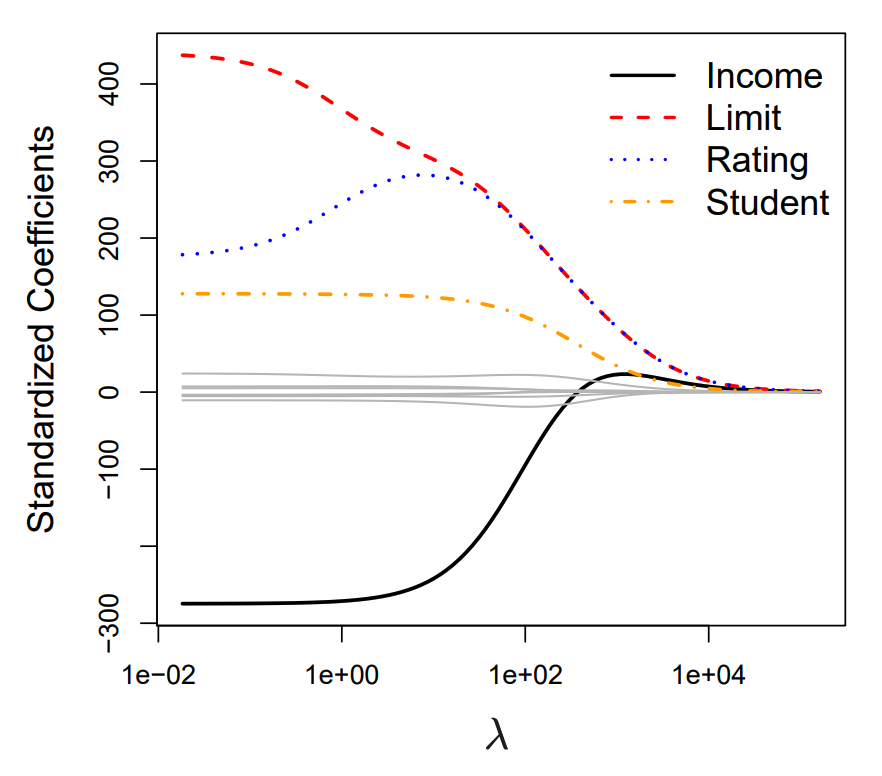
\includegraphics[width=4cm]{data/ridge.png}
            };

            \node[] at (-2.5, -2.5) {};
            \node[] at (7.5, 2.5) {};
        \end{tikzpicture}
        \vfill
    \end{frame}

    \begin{frame}{Shrinkage: LASSO} % Lasso coefficients
        \vfill
        \centering
        \begin{tikzpicture}
            \node[fill=white, draw=black, label=Ridge] at (0, 0) {
                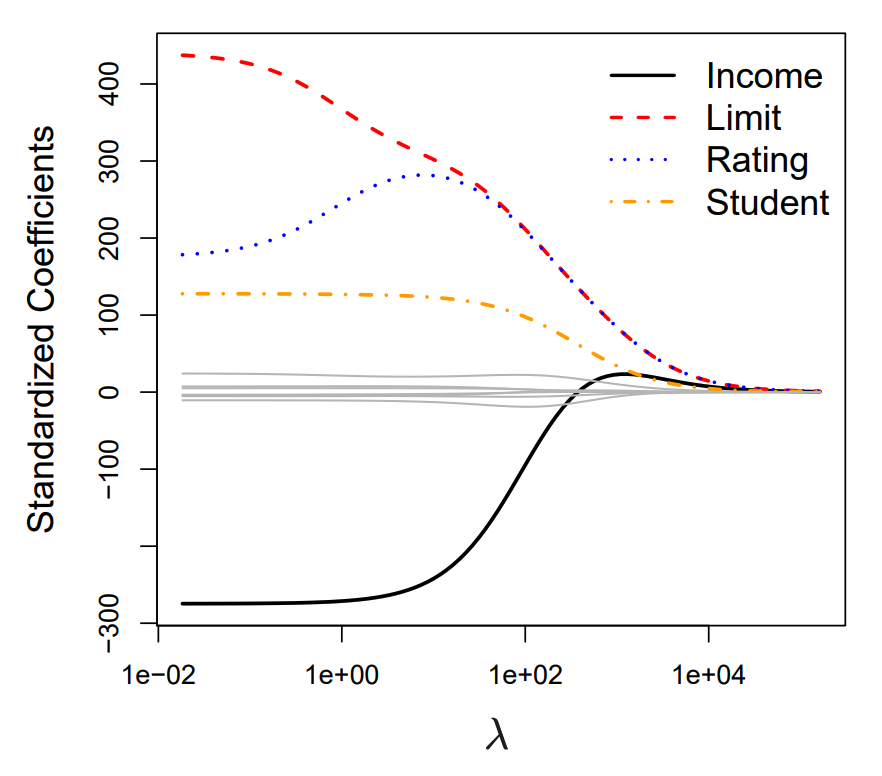
\includegraphics[width=4cm]{data/ridge.png}
            };
            \node[fill=white, draw=black, label=LASSO] at (5, 0) {
                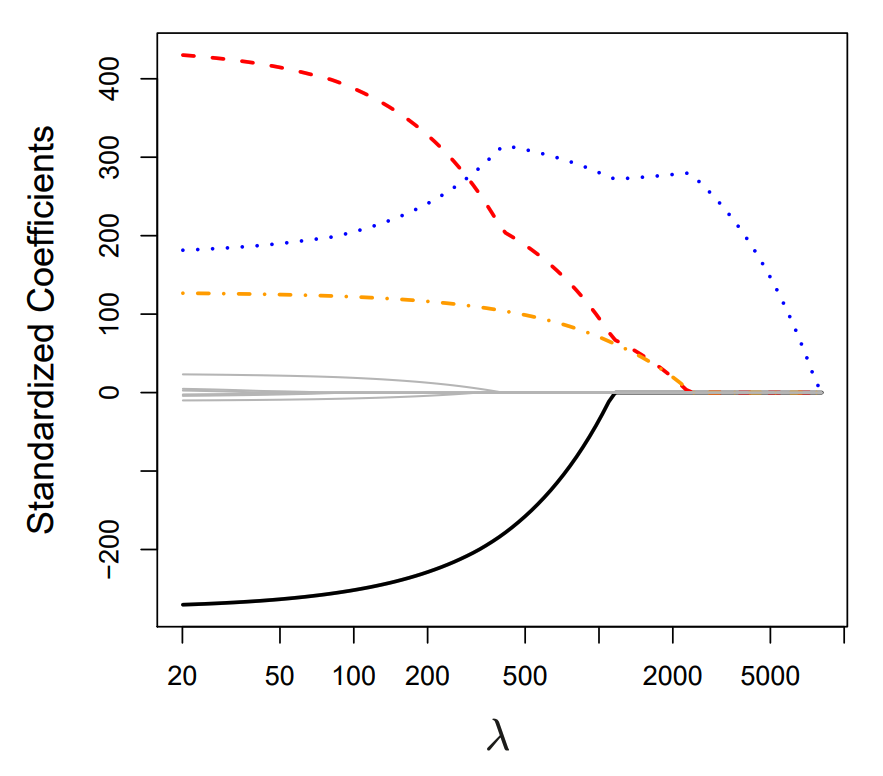
\includegraphics[width=4cm]{data/lasso.png}
            };

            \node[] at (-2.5, -2.5) {};
            \node[] at (7.5, 2.5) {};
        \end{tikzpicture}
        \vfill
    \end{frame}

    \begin{frame}{Shrinkage: LASSO}
        \centering
        \vfill
        \begin{tabular}{|c|c|c|}
            \hline
            \textbf{Predictor}&\textbf{Ridge}&\textbf{LASSO}\\
            \hline
            Intercept&23.44&23.44\\
            \hline
            Weight&-5.59&-4.78\\
            \hline
            Year&2.75&2.00\\
            \hline
            Horsepower&-0.07&-0.09\\
            \hline
            Cylinders&-0.54&0\\
            \hline
            Acceleration&0.19&0\\
            \hline
            Displacement&0.66&0\\
            \hline
        \end{tabular}
        \vfill
    \end{frame}

    \begin{frame}{Shrinkage: LASSO}
        \vfill
        \centering
        \begin{tikzpicture}
            \node[fill=white, draw=black] at (0, 0) {
                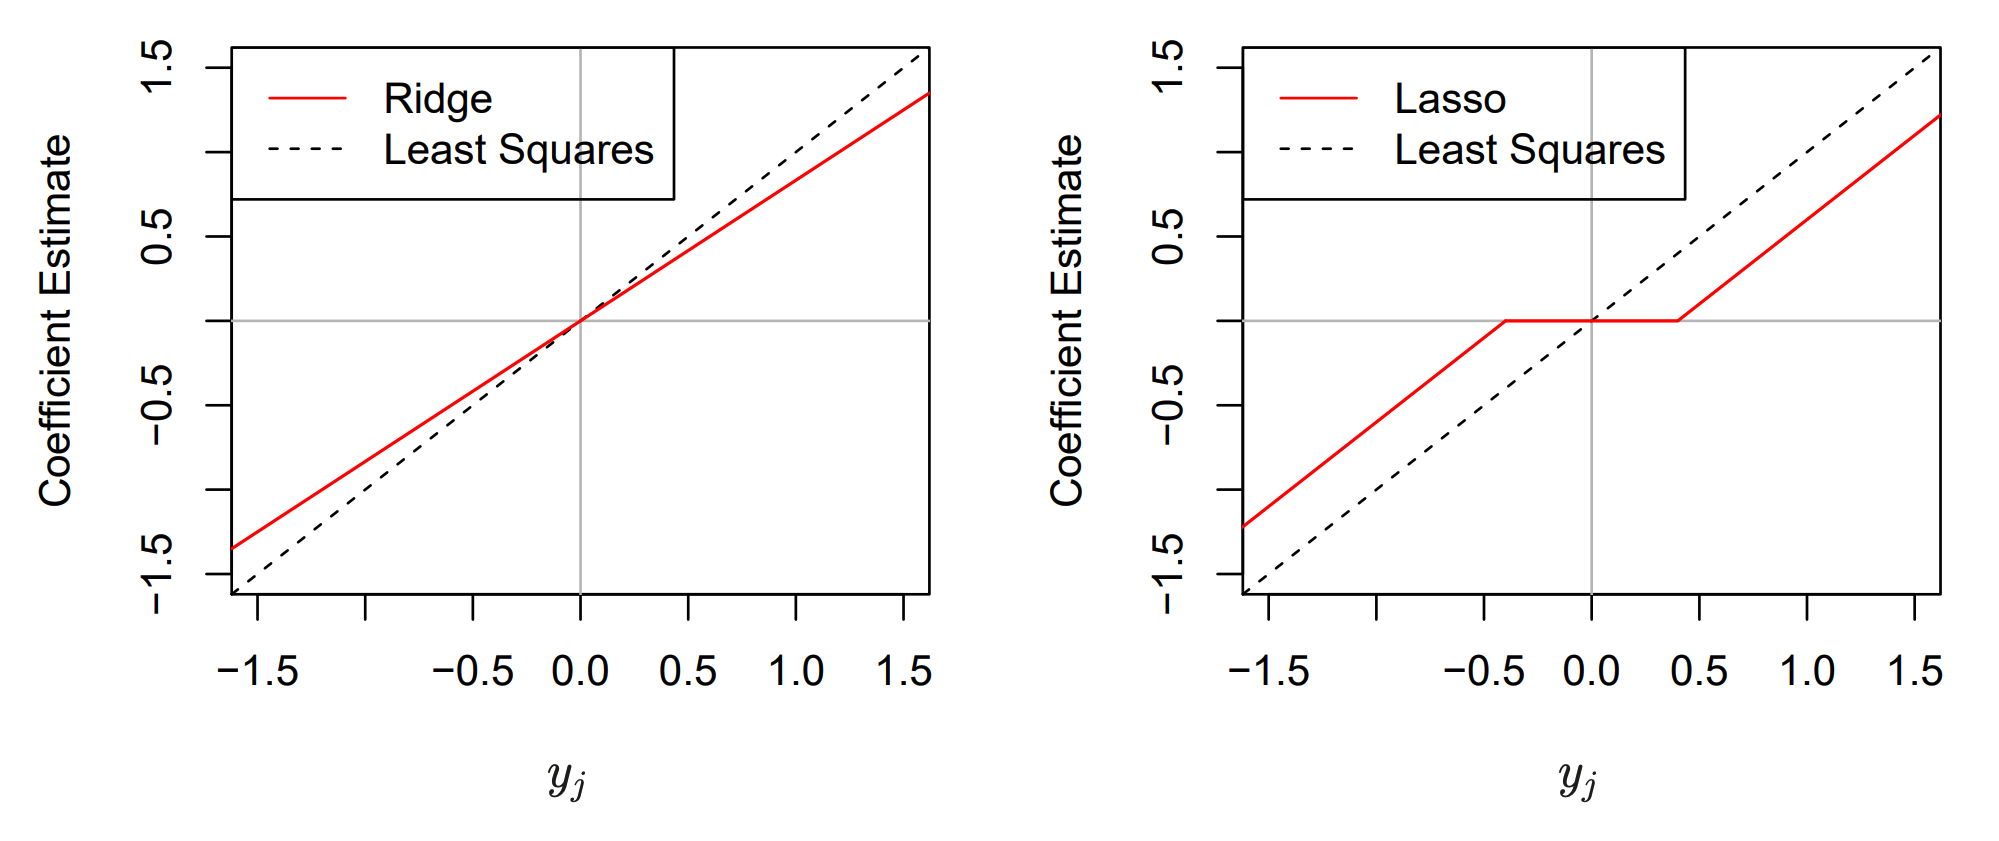
\includegraphics[width=10cm]{data/ridge_vs_lasso.png}
            };
        \end{tikzpicture}
        \vfill
    \end{frame}

    \begin{frame}{Shrinkage: LASSO}
        \vfill
        \centering
        \begin{tikzpicture}
            \node[fill=white, draw=black] at (0, 0) {
                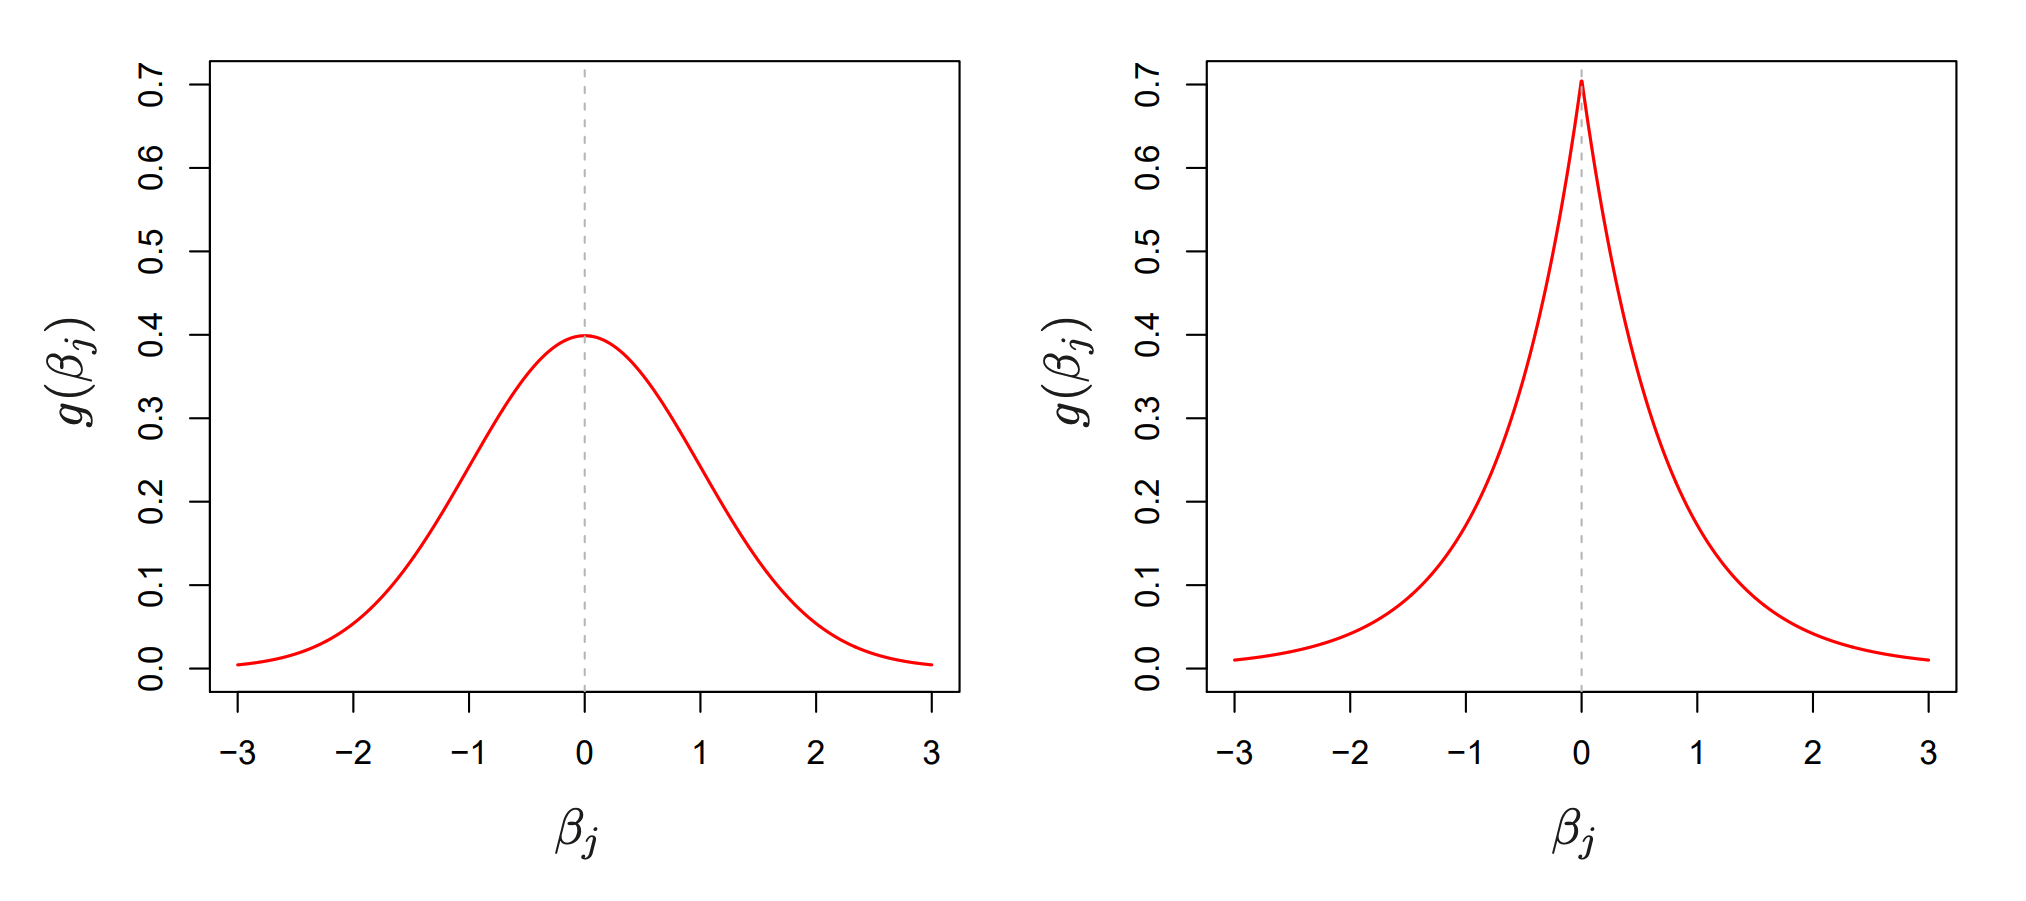
\includegraphics[width=9.5cm]{data/shrinkage_priors.png}
            };
        \end{tikzpicture}
        \vfill
    \end{frame}

    \begin{frame}{Shrinkage: Summary} % MSE
        \centering
        \vfill
        \begin{tikzpicture}
            \node[inner sep=0pt] (mse) at (0, 2.2) {
                $= \sum\limits_{i=0}^n \left( y_i - \sum\limits_{j=0}^p \beta_j x_{ij} \right)^2$
            };
            \node[anchor=east, inner sep=0pt] at (mse.west) {
                $loss_{mse}$
            };

            \node[anchor=west, align=left] at ($ (mse.west) + (4.7, 0) $) {Fits the \textbf{best} model\\to the data.};

            \node[] at (-3, -4) {};
            \node[] at (6.8, 3) {};

            \draw[black] (3.2, 3) -- (3.2, -3.9);
        \end{tikzpicture}
        \vfill
    \end{frame}

    \begin{frame}{Shrinkage: Summary} % Ridge
        \centering
        \vfill
        \begin{tikzpicture}
            \node[inner sep=0pt] (mse) at (0, 2.2) {
                $= \sum\limits_{i=0}^n \left( y_i - \sum\limits_{j=0}^p \beta_j x_{ij} \right)^2$
            };
            \node[anchor=east, inner sep=0pt] at (mse.west) {
                $loss_{mse}$
            };


            \node[inner sep=0pt] (ridgemse) at (0, 0) {
                $= \sum\limits_{i=0}^n \left( y_i - \sum\limits_{j=0}^p \beta_j x_{ij} \right)^2$
            };
            \node[anchor=west, inner sep=0pt] (lasso) at (ridgemse.east) {
                $ + \lambda \sum\limits_{j=0}^p \beta_j^2$
            };
            \node[anchor=east, inner sep=0pt] at (ridgemse.west) {
                $loss_{ridge}$
            };


            \node[anchor=west, align=left] at ($ (mse.west) + (4.7, 0) $) {Fits the \textbf{best} model\\to the data.};
            \node[anchor=west, align=left] at ($ (ridgemse.west) + (4.7, 0) $) {Fits the \textbf{best} model\\to the data while\\\textbf{shrinking} coefficients\\towards zero.};

            \node[] at (-3, -4) {};
            \node[] at (6.8, 3) {};

            \draw[black] (3.2, 3) -- (3.2, -3.9);
        \end{tikzpicture}
        \vfill
    \end{frame}

    \begin{frame}{Shrinkage: Summary} % LASSO
        \centering
        \vfill
        \begin{tikzpicture}
            \node[inner sep=0pt] (mse) at (0, 2.2) {
                $= \sum\limits_{i=0}^n \left( y_i - \sum\limits_{j=0}^p \beta_j x_{ij} \right)^2$
            };
            \node[anchor=east, inner sep=0pt] at (mse.west) {
                $loss_{mse}$
            };


            \node[inner sep=0pt] (ridgemse) at (0, 0) {
                $= \sum\limits_{i=0}^n \left( y_i - \sum\limits_{j=0}^p \beta_j x_{ij} \right)^2$
            };
            \node[anchor=west, inner sep=0pt] (lasso) at (ridgemse.east) {
                $ + \lambda \sum\limits_{j=0}^p \beta_j^2$
            };
            \node[anchor=east, inner sep=0pt] at (ridgemse.west) {
                $loss_{ridge}$
            };


            \node[inner sep=0pt] (lassomse) at (0, -2.2) {
                $= \sum\limits_{i=0}^n \left( y_i - \sum\limits_{j=0}^p \beta_j x_{ij} \right)^2$
            };
            \node[anchor=west, inner sep=0pt] (lasso) at (lassomse.east) {
                $ + \lambda \sum\limits_{j=0}^p |\beta_j|$
            };
            \node[anchor=east, inner sep=0pt] at (lassomse.west) {
                $loss_{lasso}$
            };

            \node[anchor=west, align=left] at ($ (mse.west) + (4.7, 0) $) {Fits the \textbf{best} model\\to the data.};
            \node[anchor=west, align=left] at ($ (ridgemse.west) + (4.7, 0) $) {Fits the \textbf{best} model\\to the data while\\\textbf{shrinking} coefficients\\towards zero.};
            \node[anchor=west, align=left] at ($ (lassomse.west) + (4.7, 0) $) {Fits the \textbf{best} model\\to the data while\\\textbf{shrinking} coefficients\\towards zero such\\that some variables\\are effectively \textbf{removed}.};

            \node[] at (-3, -4) {};
            \node[] at (6.8, 3) {};

            \draw[black] (3.2, 3) -- (3.2, -3.9);
        \end{tikzpicture}
        \vfill
    \end{frame}

    \section{Dimensionality reduction}

    \begin{frame}{Dimensionality reduction: Motivation}
        \centering
        Although we have $p$ predictors, there are actually $q<p$ dimensions of variability in our data, and using $q$ instead of $p$ is going to reduce model complexity.
    \end{frame}

    \begin{frame}{Dimensionality reduction: Outline}
        \centering
        \vfill
        \begin{tikzpicture}
            \begin{groupplot}[
                group style={
                    group size=3 by 2,
                    horizontal sep=0.5cm
                },
                ticklabel style = {font=\tiny},
                height=3.9cm,
                width=3.9cm
            ]
                \newcommand{\autoplot}[1]{
                    \nextgroupplot[
                        title=\scriptsize{####1},
                        every axis title/.style={at={(0.5,1.15)}},
                        xtick pos=bottom,
                        ytick pos=left
                    ]
                        \addplot[
                            only marks,
                            mark=*,
                            color=blue,
                            opacity=0.25
                        ] table[
                            col sep=comma,
                            y=mpg,
                            x=####1
                        ] {data/Auto.csv};
                }
                \autoplot{cylinders}
                \autoplot{displacement}
                \autoplot{horsepower}
                \autoplot{weight}
                \autoplot{acceleration}
                \autoplot{year}
            \end{groupplot}

        \end{tikzpicture}
        \vfill
    \end{frame}

    \begin{frame}{Dimensionality reduction: Principal component analysis} % Heatmap
        \begin{tikzpicture}
            \begin{axis}[
                colormap/hot, % You can choose a different colormap
                colorbar,
                axis on top,
                xlabel=X-axis Label,
                ylabel=Y-axis Label,
            ]
            \end{axis}
        \end{tikzpicture}
    \end{frame}

    \begin{frame}{Dimensionality reduction: Principal component analysis} % 2 variables
        \centering
        \vfill
        \begin{tikzpicture}
            \begin{axis}[
                height=7cm,
                width=7cm,
                xlabel=weight,
                ylabel=horsepower,
                xmin=-2,
                xmax=3.5,
                ymin=-2,
                ymax=3
            ]
                \addplot[
                    only marks,
                    mark=*,
                    color=blue,
                    opacity=0.05
                ] table [col sep=comma, x=x, y=y] {data/components.csv};
            \end{axis}
        \end{tikzpicture}
        \vfill
    \end{frame}


    \begin{frame}{Dimensionality reduction: Principal component analysis} % Center
        \centering
        \vfill
        \begin{tikzpicture}
            \begin{axis}[
                height=7cm,
                width=7cm,
                xlabel=weight,
                ylabel=horsepower,
                xmin=-2,
                xmax=3.5,
                ymin=-2,
                ymax=3
            ]
                \addplot[
                    only marks,
                    mark=*,
                    color=blue,
                    opacity=0.05
                ] table [col sep=comma, x=x, y=y] {data/components.csv};
                \addplot[only marks, mark=*, color=red] coordinates {
                    (-1.81260902e-16, -1.81260902e-17)
                };
            \end{axis}
        \end{tikzpicture}
        \vfill
    \end{frame}

    \begin{frame}{Dimensionality reduction: Principal component analysis} % First direction
        \centering
        \vfill
        \begin{tikzpicture}
            \begin{axis}[
                height=7cm,
                width=7cm,
                xlabel=weight,
                ylabel=horsepower,
                xmin=-2,
                xmax=3.5,
                ymin=-2,
                ymax=3
            ]
                \addplot[
                    only marks,
                    mark=*,
                    color=blue,
                    opacity=0.05
                ] table [col sep=comma, x=x, y=y] {data/components.csv};
                \addplot[only marks, mark=*, color=red] coordinates {
                    (-1.81260902e-16, -1.81260902e-17)
                };
                \draw[red,-Latex,very thick] (axis cs: -1.81260902e-16, -1.81260902e-17) -- (axis cs: -1.81260902e-16 + 0.96677463, -1.81260902e-17 + 0.96677463);
            \end{axis}
        \end{tikzpicture}
        \vfill
    \end{frame}

    \begin{frame}{Dimensionality reduction: Principal component analysis} % First PC
        \centering
        \vfill
        \begin{tikzpicture}
            \begin{axis}[
                height=7cm,
                width=7cm,
                xlabel=weight,
                ylabel=horsepower,
                xmin=-2,
                xmax=3.5,
                ymin=-2,
                ymax=3
            ]
                \addplot[
                    only marks,
                    mark=*,
                    color=blue,
                    opacity=0.05
                ] table [col sep=comma, x=x, y=y] {data/components.csv};
                \addplot[only marks, mark=*, color=red] coordinates {
                    (-1.81260902e-16, -1.81260902e-17)
                };
                \draw[red,-Latex,very thick] (axis cs: -1.81260902e-16 - 5 * 0.96677463, -1.81260902e-17 - 5 * 0.96677463) -- (axis cs: -1.81260902e-16 + 5 * 0.96677463, -1.81260902e-17 + 5 * 0.96677463);
                \draw[red,|-|,very thick] (axis cs: -1.81260902e-16 - 1 * 0.96677463, -1.81260902e-17 - 1 * 0.96677463) -- (axis cs: -1.81260902e-16 + 1 * 0.96677463, -1.81260902e-17 + 1 * 0.96677463);
                \draw[red,|-|,very thick] (axis cs: -1.81260902e-16 - 2 * 0.96677463, -1.81260902e-17 - 2 * 0.96677463) -- (axis cs: -1.81260902e-16 + 2 * 0.96677463, -1.81260902e-17 + 2 * 0.96677463);

                \node[rotate=45, anchor=north, inner sep=5pt] at (axis cs: -1.81260902e-16 - 1 * 0.96677463, -1.81260902e-17 - 1 * 0.96677463) {\Large{\textbf{\textcolor{red}{-1}}}};
                \node[rotate=45, anchor=north, inner sep=5pt] at (axis cs: -1.81260902e-16 - 2 * 0.96677463, -1.81260902e-17 - 2 * 0.96677463) {\Large{\textbf{\textcolor{red}{-2}}}};
                \node[rotate=45, anchor=north, inner sep=5pt] at (axis cs: -1.81260902e-16 + 1 * 0.96677463, -1.81260902e-17 + 1 * 0.96677463) {\Large{\textbf{\textcolor{red}{1}}}};
                \node[rotate=45, anchor=north, inner sep=5pt] at (axis cs: -1.81260902e-16 + 2 * 0.96677463, -1.81260902e-17 + 2 * 0.96677463) {\Large{\textbf{\textcolor{red}{2}}}};
                \node[rotate=45, anchor=south, inner sep=3pt] at (axis cs: -1.81260902e-16 + 2.5 * 0.96677463, -1.81260902e-17 + 2.5 * 0.96677463) {\Large{\textbf{\textcolor{red}{PC1}}}};
            \end{axis}
        \end{tikzpicture}
        \vfill
    \end{frame}

    \begin{frame}{Dimensionality reduction: Principal component analysis} % Second direction
        \centering
        \vfill
        \begin{tikzpicture}
            \begin{axis}[
                height=7cm,
                width=7cm,
                xlabel=weight,
                ylabel=horsepower,
                xmin=-2,
                xmax=3.5,
                ymin=-2,
                ymax=3
            ]
                \addplot[
                    only marks,
                    mark=*,
                    color=blue,
                    opacity=0.05
                ] table [col sep=comma, x=x, y=y] {data/components.csv};
                \addplot[only marks, mark=*, color=red] coordinates {
                    (-1.81260902e-16, -1.81260902e-17)
                };
                \draw[red,-Latex,very thick] (axis cs: -1.81260902e-16 - 5 * 0.96677463, -1.81260902e-17 - 5 * 0.96677463) -- (axis cs: -1.81260902e-16 + 5 * 0.96677463, -1.81260902e-17 + 5 * 0.96677463);
                \draw[red,|-|,very thick] (axis cs: -1.81260902e-16 - 1 * 0.96677463, -1.81260902e-17 - 1 * 0.96677463) -- (axis cs: -1.81260902e-16 + 1 * 0.96677463, -1.81260902e-17 + 1 * 0.96677463);
                \draw[red,|-|,very thick] (axis cs: -1.81260902e-16 - 2 * 0.96677463, -1.81260902e-17 - 2 * 0.96677463) -- (axis cs: -1.81260902e-16 + 2 * 0.96677463, -1.81260902e-17 + 2 * 0.96677463);

                \node[rotate=45, anchor=north, inner sep=5pt] at (axis cs: -1.81260902e-16 - 1 * 0.96677463, -1.81260902e-17 - 1 * 0.96677463) {\Large{\textbf{\textcolor{red}{-1}}}};
                \node[rotate=45, anchor=north, inner sep=5pt] at (axis cs: -1.81260902e-16 - 2 * 0.96677463, -1.81260902e-17 - 2 * 0.96677463) {\Large{\textbf{\textcolor{red}{-2}}}};
                \node[rotate=45, anchor=north, inner sep=5pt] at (axis cs: -1.81260902e-16 + 1 * 0.96677463, -1.81260902e-17 + 1 * 0.96677463) {\Large{\textbf{\textcolor{red}{1}}}};
                \node[rotate=45, anchor=north, inner sep=5pt] at (axis cs: -1.81260902e-16 + 2 * 0.96677463, -1.81260902e-17 + 2 * 0.96677463) {\Large{\textbf{\textcolor{red}{2}}}};
                \node[rotate=45, anchor=south, inner sep=3pt] at (axis cs: -1.81260902e-16 + 2.5 * 0.96677463, -1.81260902e-17 + 2.5 * 0.96677463) {\Large{\textbf{\textcolor{red}{PC1}}}};

                \draw[red,-Latex,very thick] (axis cs: -1.81260902e-16, -1.81260902e-17) -- (axis cs: -1.81260902e-16 + 3 * 0.26058464, -1.81260902e-17 - 3 * 0.26058464);
            \end{axis}
        \end{tikzpicture}
        \vfill
    \end{frame}

    \begin{frame}{Dimensionality reduction: Principal component analysis} % Second PC
        \centering
        \vfill
        \begin{tikzpicture}
            \begin{axis}[
                height=7cm,
                width=7cm,
                xlabel=weight,
                ylabel=horsepower,
                xmin=-2,
                xmax=3.5,
                ymin=-2,
                ymax=3
            ]
                \addplot[
                    only marks,
                    mark=*,
                    color=blue,
                    opacity=0.05
                ] table [col sep=comma, x=x, y=y] {data/components.csv};
                \addplot[only marks, mark=*, color=red] coordinates {
                    (-1.81260902e-16, -1.81260902e-17)
                };
                \draw[red,-Latex,very thick] (axis cs: -1.81260902e-16 - 5 * 0.96677463, -1.81260902e-17 - 5 * 0.96677463) -- (axis cs: -1.81260902e-16 + 5 * 0.96677463, -1.81260902e-17 + 5 * 0.96677463);
                \draw[red,|-|,very thick] (axis cs: -1.81260902e-16 - 1 * 0.96677463, -1.81260902e-17 - 1 * 0.96677463) -- (axis cs: -1.81260902e-16 + 1 * 0.96677463, -1.81260902e-17 + 1 * 0.96677463);
                \draw[red,|-|,very thick] (axis cs: -1.81260902e-16 - 2 * 0.96677463, -1.81260902e-17 - 2 * 0.96677463) -- (axis cs: -1.81260902e-16 + 2 * 0.96677463, -1.81260902e-17 + 2 * 0.96677463);

                \node[rotate=45, anchor=north, inner sep=5pt] at (axis cs: -1.81260902e-16 - 1 * 0.96677463, -1.81260902e-17 - 1 * 0.96677463) {\Large{\textbf{\textcolor{red}{-1}}}};
                \node[rotate=45, anchor=north, inner sep=5pt] at (axis cs: -1.81260902e-16 - 2 * 0.96677463, -1.81260902e-17 - 2 * 0.96677463) {\Large{\textbf{\textcolor{red}{-2}}}};
                \node[rotate=45, anchor=north, inner sep=5pt] at (axis cs: -1.81260902e-16 + 1 * 0.96677463, -1.81260902e-17 + 1 * 0.96677463) {\Large{\textbf{\textcolor{red}{1}}}};
                \node[rotate=45, anchor=north, inner sep=5pt] at (axis cs: -1.81260902e-16 + 2 * 0.96677463, -1.81260902e-17 + 2 * 0.96677463) {\Large{\textbf{\textcolor{red}{2}}}};
                \node[rotate=45, anchor=south, inner sep=3pt] at (axis cs: -1.81260902e-16 + 2.5 * 0.96677463, -1.81260902e-17 + 2.5 * 0.96677463) {\Large{\textbf{\textcolor{red}{PC1}}}};

                \draw[red,|-|,very thick] (axis cs: -1.81260902e-16 - 1 * 0.26058464, -1.81260902e-17 + 1 * 0.26058464) -- (axis cs: -1.81260902e-16 + 1 * 0.26058464, -1.81260902e-17 - 1 * 0.26058464);
                \draw[red,|-|,very thick] (axis cs: -1.81260902e-16 - 2 * 0.26058464, -1.81260902e-17 + 2 * 0.26058464) -- (axis cs: -1.81260902e-16 + 2 * 0.26058464, -1.81260902e-17 - 2 * 0.26058464);
                \draw[red,|-|,very thick] (axis cs: -1.81260902e-16 - 3 * 0.26058464, -1.81260902e-17 + 3 * 0.26058464) -- (axis cs: -1.81260902e-16 + 3 * 0.26058464, -1.81260902e-17 - 3 * 0.26058464);
                \draw[red,|-|,very thick] (axis cs: -1.81260902e-16 - 4 * 0.26058464, -1.81260902e-17 + 4 * 0.26058464) -- (axis cs: -1.81260902e-16 + 4 * 0.26058464, -1.81260902e-17 - 4 * 0.26058464);
                \draw[red,|-|,very thick] (axis cs: -1.81260902e-16 - 5 * 0.26058464, -1.81260902e-17 + 5 * 0.26058464) -- (axis cs: -1.81260902e-16 + 5 * 0.26058464, -1.81260902e-17 - 5 * 0.26058464);
                \draw[red,|-|,very thick] (axis cs: -1.81260902e-16 - 6 * 0.26058464, -1.81260902e-17 + 6 * 0.26058464) -- (axis cs: -1.81260902e-16 + 6 * 0.26058464, -1.81260902e-17 - 6 * 0.26058464);
                \draw[red,|-|,very thick] (axis cs: -1.81260902e-16 - 7 * 0.26058464, -1.81260902e-17 + 7 * 0.26058464) -- (axis cs: -1.81260902e-16 + 7 * 0.26058464, -1.81260902e-17 - 7 * 0.26058464);
                \draw[red,|-|,very thick] (axis cs: -1.81260902e-16 - 8 * 0.26058464, -1.81260902e-17 + 8 * 0.26058464) -- (axis cs: -1.81260902e-16 + 8 * 0.26058464, -1.81260902e-17 - 8 * 0.26058464);
                \draw[red,|-|,very thick] (axis cs: -1.81260902e-16 - 9 * 0.26058464, -1.81260902e-17 + 9 * 0.26058464) -- (axis cs: -1.81260902e-16 + 9 * 0.26058464, -1.81260902e-17 - 9 * 0.26058464);
            \end{axis}
        \end{tikzpicture}
        \vfill
    \end{frame}

    \begin{frame}{Dimensionality reduction: Principal component analysis} % PC space
        \centering
        \vfill
        \begin{tikzpicture}
            \begin{axis}[
                height=7cm,
                width=7cm,
                xlabel=PC1,
                ylabel=PC2,
            ]
                \addplot[
                    only marks,
                    mark=*,
                    color=blue,
                    opacity=0.25
                ] table [col sep=comma, x=x, y=y] {data/pcs.csv};
            \end{axis}
        \end{tikzpicture}
        \vfill
    \end{frame}

    \begin{frame}[t]{Dimensionality reduction: Principal component regression} % Table
        \centering
        \vspace{1cm}
        \begin{tabular}{|c|c|c|c|c|}
            \hline
            \textbf{mpg}&\textbf{horsepower}&\textbf{weight}&\textbf{PC1}&\textbf{PC2}\\
            \hline
            18&130&3504&0.908&0.303\\
            \hline
            15&165&3693&1.709&0.517\\
            \hline
            18&150&3436&1.219&0.455\\
            \hline
            16&150&3433&1.217&0.457\\
            \hline
            17&140&3449&1.046&0.260\\
            \hline
            15&198&4341&2.856&0.583\\
            \hline
            14&220&4354&3.272&0.977\\
            \hline
        \end{tabular}
    \end{frame}

    \begin{frame}[t]{Dimensionality reduction: Principal component analysis} % Regular OLS
        \centering
        \vspace{1cm}
        \begin{tabular}{|c|c|c|c|c|}
            \hline
            \textbf{mpg}&\textbf{horsepower}&\textbf{weight}&\textbf{PC1}&\textbf{PC2}\\
            \hline
            18&130&3504&0.908&0.303\\
            \hline
            15&165&3693&1.709&0.517\\
            \hline
            18&150&3436&1.219&0.455\\
            \hline
            16&150&3433&1.217&0.457\\
            \hline
            17&140&3449&1.046&0.260\\
            \hline
            15&198&4341&2.856&0.583\\
            \hline
            14&220&4354&3.272&0.977\\
            \hline
        \end{tabular}\\
        \vspace{0.5cm}
        $mpg \sim \beta_0 + \beta_1 * horsepower + \beta_2 * weight$\\
    \end{frame}

    \begin{frame}[t]{Dimensionality reduction: Principal component analysis} % PCR
        \centering
        \vspace{1cm}
        \begin{tabular}{|c|c|c|c|c|}
            \hline
            \textbf{mpg}&\textbf{horsepower}&\textbf{weight}&\textbf{PC1}&\textbf{PC2}\\
            \hline
            18&130&3504&0.908&0.303\\
            \hline
            15&165&3693&1.709&0.517\\
            \hline
            18&150&3436&1.219&0.455\\
            \hline
            16&150&3433&1.217&0.457\\
            \hline
            17&140&3449&1.046&0.260\\
            \hline
            15&198&4341&2.856&0.583\\
            \hline
            14&220&4354&3.272&0.977\\
            \hline
        \end{tabular}\\
        \vspace{0.5cm}
        $mpg \sim \beta_0 + \beta_1 * horsepower + \beta_2 * weight$\\
        \vspace{0.25cm}
        $mpg \sim \beta_0 + \beta_1 * PC1 + \beta_2 * PC2$
    \end{frame}

    \begin{frame}{Dimensionality reduction: Principal component analysis}
        \underline{Principal component regression}
        \begin{enumerate}
            \item Fit a PCA to transform your $p$ predictors into $p$ principal components.
            \item Fit a linear regression model using a subset of the principal components.
        \end{enumerate}
        \vspace{0.25cm}
        \underline{\textcolor{green}{+} Positives}\\
        \begin{itemize}
            \item The principal components are orthogonal, so there is no issue of collinearity.\\
            \item The principal components are ordered by the amount of variance they explain, so we can select the early principal components to explain most of the variability in the predictors.\\
        \end{itemize}
        \vspace{0.25cm}
        \underline{\textcolor{red}{-} Drawbacks}\\
        \begin{itemize}
            \item Have to select number of principal components to use.
            \item What if the principal components that explain the largest amount of variance as not related to the outcome?
        \end{itemize}
        \end{frame}

    \begin{frame}{Dimensionality reduction: Partial least squares}
        Next time
    \end{frame}
\end{document}
